\chapter{全纯函数的积分表示\label{chap3}}

本章将要介绍的Cauchy积分定理和Cauchy积分公式是整个全纯函数理论的基础,由它们可以推出一系列重要的结论,
例如全纯函数有任意阶导数,而且可以展开成幂级数等. 其中,Cauchy积分定理又是最根本的.


\section{复变函数的积分\label{sec3.1}}

设$z=\gamma(t)$($a\le t\le b$)是一条可求长曲线,$f$是定义在$\gamma$上的函数,
沿$\gamma$的正方向取分点$\gamma(a)=z_0,z_1,z_2,\cdots,z_n=\gamma(b)$,
在$\gamma$中从$z_{k-1}$到$z_k$的弧段上任取点$\zeta_k$, $k=1,\cdots,n$(见图 \ref{fig3.1}),作Riemann和
\begin{equation}\label{eq3.1.1}
  \sum_{k=1}^n f(\zeta_k) (z_k - z_{k-1}).
\end{equation}
\begin{figure}[!ht]
  \centering
  \begin{tikzpicture}[thick,>=Stealth]
    \draw(-4,0)node[below]{$z_0=\gamma(a)$}arc(180:90:4)node[right]{$z_n=\gamma(b)$};
    \foreach \x in {180,170,155,140,130,125,120,105,90}
      \fill(\x:4)circle(1pt);
    \draw(170:4)node[left]{$z_1$}(130:4)node[above left]{$z_{k-1}$}
         (125:4)node[below right]{$\zeta_k$}(120:4)node[above left]{$z_k$};
  \end{tikzpicture}
  \caption{\label{fig3.1}}
\end{figure}
用$s_k$记弧段$\wideparen{z_{k-1}z_k}$的长度,如果当$\lambda=\max\{s_k:1\le k\le n\}\to0$时,不论$\zeta_k$的取法如何,和式 \eqref{eq3.1.1} 总有一确定的极限,就称此极限为$f$沿
$\gamma$的积分,记为$\int\limits_\gamma f(z)\dz$,即
\[
  \int\limits_\gamma f(z)\dz = \lim_{\lambda\to0}\sum_{k=1}^nf(\zeta_k)(z_k-z_{k-1}).
\]

什么情况下上述极限存在呢?事实上,只要$f$在$\gamma$上连续,上述积分一定存在.为了证明这一点,记$z_k=x_k+\ii y_k,\zeta_k=\xi_k+\ii\eta_k,f(\zeta_k)=u(\xi_k,\eta_k)+\ii v(\xi_k,\eta_k)$,于是和式 \eqref{eq3.1.1} 便可写成
\[
  \sum_{k=1}^n\{u(\xi_k,\eta_k)\Delta x_k-v(\xi_k,\eta_k)\Delta y_k\}
  +\ii\sum_{k=1}^n\{v(\xi_k,\eta_k)\Delta x_k+u(\xi_k,\eta_k)\Delta y_k\},
\]
这里,$\Delta x_k=x_k-x_{k-1},\Delta y_k=y_k-y_{k-1}$. 当$u,v$在$\gamma$上连续时,上述和当$\lambda\to0$时趋于曲线积分
\[
  \int\limits_\gamma u\dx-v\dy+\ii\int\limits_\gamma v\dx+u\dy.
\]
这样,我们就证明了
\begin{prop}\label{prop3.1.1}
设$f=u+\ii v$在可求长曲线$\gamma$上连续,则有
\begin{equation}\label{eq3.1.2}
  \int\limits_\gamma f(z)\dz=\int\limits_\gamma u\dx-v\dy+\ii\int\limits_\gamma v\dx+u\dy.
\end{equation}
\end{prop}

这个公式通过下面的形式计算很容易记住:
\begin{align*}
  f(z)\dz & = (u+\ii v)(\dx+\ii\dy) \\
          & = (u\dx-v\dy)+\ii(v\dx+u\dy).
\end{align*}

如果曲线是光滑的,还可以通过曲线的参数方程来计算积分.
\begin{prop}\label{prop3.1.2}
  如果$z=\gamma(t)$($a\le t\le b$)是光滑曲线,$f$在$\gamma$上连续,那么
  \begin{equation}\label{eq3.1.3}
    \int\limits_\gamma f(z)\dz = \int_a^b f\big(\gamma(t)\big)\gamma'(t)\dif t.
  \end{equation}
\end{prop}
\begin{proof}
  设$z=\gamma(t)=x(t)+\ii y(t)$,在所设的条件下,有
  \begin{align*}
    & \int\limits_\gamma u\dx-v\dy = \int_a^b\big[u\big(x(t),y(t)\big)x'(t)-v\big(x(t),y(t)\big)y'(t)\big]\dif t,\\
    & \int\limits_\gamma v\dx+u\dy = \int_a^b\big[v\big(x(t),y(t)\big)x'(t)+u\big(x(t),y(t)\big)y'(t)\big]\dif t.
  \end{align*}
  第二式乘$\ii$后与第一式相加,即得
  \begin{align*}
    \int\limits_\gamma f(z)\dz
    & = \int_a^b \big[u\big(x(t),y(t)\big)+\ii v\big(x(t),y(t)\big)\big]\big(x'(t)+\ii y'(t)\big)\dif t\\
    & = \int_a^b f\big(\gamma(t)\big)\gamma'(t)\dif t. \qedhere
  \end{align*}
\end{proof}
\begin{example}\label{exam3.1.3}
  设可求长曲线$z=\gamma(t)$($a\le t\le b$)的起点为$\alpha$,终点为$\beta$,证明:
  \begin{align*}
    & \int\limits_\gamma\dz = \beta-\alpha,\\
    & \int\limits_\gamma z\dz = \frac12(\beta^2-\alpha^2).
  \end{align*}
\end{example}
\begin{proof}
  若$\gamma$是光滑曲线,由公式 \eqref{eq3.1.3},得
  \begin{align*}
    & \int\limits_\gamma \dz = \int_a^b\gamma'(t)\dif t=\gamma(b)-\gamma(a)=\beta-\alpha,\\
    & \int\limits_\gamma z\dz = \int_a^b\gamma(t)\gamma'(t)\dif t
      = \frac12\gamma^2(t)\bigg|_a^b = \frac12\big(\gamma^2(b)-\gamma^2(a)\big)
      = \frac12(\beta^2-\alpha^2).
  \end{align*}
  如果$\gamma$不是光滑曲线,可直接按积分的定义计算:
  \begin{align*}
  &\int\limits_\gamma\dz=\lim_{\lambda\to0}\sum_{k=1}^n(z_k-z_{k-1})
  =z_n-z_0=\beta-\alpha.\\
  &\int\limits_\gamma z\dz=\lim_{\lambda\to0}\sum_{k=1}^nz_k(z_k-z_{k-1}),\\
  &\int\limits_\gamma z\dz=\lim_{\lambda\to0}\sum_{k=1}^nz_{k-1}(z_k-z_{k-1}),
  \end{align*}
  把两式加起来,得
  \begin{equation*}
    \int\limits_\gamma z\dz=\frac12\lim_{\lambda\to0}
    \sum_{k=1}^n(z_k^2-z_{k-1}^2)=\frac12(z_n^2-z_0^2)=\frac12(\beta^2-\alpha^2). \qedhere
  \end{equation*}
\end{proof}

\begin{example}\label{exam3.1.4}
  计算积分$\int\limits_\gamma\frac{\dz}{(z-a)^n}$,这里,$n$是任意整数,
$\gamma$是以$a$为中心、以$r$为半径的圆周.
\end{example}
\begin{solution}
  $\gamma$的参数方程为$z=a+r\ee^{\ii t},0\le t\le2\pi$. 由公式 \eqref{eq3.1.3},得
  \[
    \int\limits_\gamma\frac{\dz}{(z-a)^n} = \int_0^{2\pi}\frac{r\ii\ee^{\ii t}}{r^n\ee^{\ii nt}}\dif t=r^{1-n}\ii\int_0^{2\pi}\ee^{\ii(1-n)t}\dif t.
  \]
  所以,上述积分当$n\ne1$时为零,当$n=1$时为$2\pi\ii$,即
  \begin{equation*}
    \int\limits_\gamma \frac{\dz}{(z-a)^n} =
    \begin{cases}
      0, & n \ne 1 ; \\
      2\pi\ii, & n = 1.
    \end{cases} \qedhere
  \end{equation*}
\end{solution}

由积分的定义,可以马上得到
\begin{prop}\label{prop3.1.5}
  如果$f,g$在可求长曲线$\gamma$上连续,那么
  \begin{eenum}
    \item \label{prop3.1.5.1} $\int\limits_{\gamma^-}f(z)\dz=-\int\limits_\gamma f(z)\dz$,这里,$\gamma^-$是指与$\gamma$方向相反的曲线;
    \item \label{prop3.1.5.2} $\int\limits_\gamma\big(\alpha f(z)+\beta g(z)\big)\dz
        =\alpha\int\limits_\gamma f(z)\dz+\beta\int\limits_\gamma g(z)\dz$,这里,$\alpha,\beta$是两个复常数;
    \item \label{prop3.1.5.3} $\int\limits_\gamma f(z)\dz=\int\limits_{\gamma_1}f(z)\dz+\int\limits_{\gamma_2}f(z)\dz$,这里,$\gamma$是由$\gamma_1$和$\gamma_2$组成的曲线.
  \end{eenum}
\end{prop}

\begin{prop}\label{prop3.1.6}
  如果$\gamma$的长度为$L,M=\sup_{z\in\gamma}|f(z)|$,那么
\begin{equation}\label{eq3.1.4}
  \bigg|\int\limits_\gamma f(z)\dz\bigg|\le ML.
\end{equation}
\end{prop}
\begin{proof}
  $f$在$\gamma$上的Riemann和有不等式
  \begin{align*}
    \bigg| \sum_{k=1}^nf(\zeta_k)(z_k-z_{k-1}) \bigg|&
    \le \sum_{k=1}^n|f(\zeta_k)|\,|z_k-z_{k-1}|\\
    & \le  M\sum_{k=1}^n|z_k-z_{k-1}|\le ML, \qedhere
  \end{align*}
令$\lambda=\max_{1\le k\le n}s_k\to0$,即得所要的表达式.
\end{proof}

这个不等式很简单,但很重要,是我们今后估计积分的主要工具,可简称为\textbf{长大不等式}.\index{B!不等式!长大不等式}

\begin{xiti}
  \item 计算积分 $\int\limits_\gamma\frac{2z-3}z\dz$,其中,$\gamma$为
    \begin{enuma}
      \item 沿圆周 $\{z:|z|=2\}$ 的上半圆,从 $-2$ 到 $2$;
      \item 沿圆周 $\{z:|z|=2\}$ 的下半圆,从 $-2$ 到 $2$;
      \item 沿圆周 $\{z:|z|=2\}$ 的正向.
    \end{enuma}
  \item 计算积分 $\int\limits_{|z|=1}\frac{\dz}{z+2}$,并证明:
    \[
      \int_0^\pi\frac{1+2\cos\theta}{5+4\cos\theta} \dif\theta = 0.
    \]
  \item 计算积分 $\int\limits_{|z|=3}\frac{2z-1}{z(z-1)}\dz$.
  \item 如果多项式 $Q(z)$ 比多项式 $P(z)$ 高两次,试证:
    \[
      \lim_{R\to\infty}\int\limits_{|z|=R}\frac{P(z)}{Q(z)}\dz = 0.
    \]
  \item 计算积分$\int\limits_{|z|=r}z^n\bar z^k\dz$,其中,$n,k$ 为整数.
  \item 设$f\in C^1(D)$,$\gamma$是域$D$中分别以$a$和$b$为起点和终点的可求长曲线. 证明:
    \[
    \int\limits_\gamma \bigg\{\pp{f(z)}z\dz + \pp{f(z)}{\bar z}\dif \bar z\bigg\} = f(b) - f(a).
    \]
  \item 设$\gamma$是可求长曲线,$\varphi$在$\gamma$上全纯,$\Gamma=\varphi(\gamma)$. 证明:
    \begin{enuma}
      \item $\Gamma$也是可求长曲线;
      \item 如果$f$在$\Gamma$上连续,那么
        \[
          \int\limits_\Gamma f(w)\dif w = \int\limits_\gamma f\big(\varphi(z)\big)\varphi'(z)\dz.
        \]
    \end{enuma}
  \item 设$\gamma$是域$D$中以$a$为起点、以$b$为终点的可求长曲线,$f,g\in H(D)\cap C^1(D)$. 证明分部积分公式:
    \[
      \int\limits_\gamma f(z)g'(z)\dz = f(z)g(z)\bigg|_a^b - \int\limits_\gamma f'(z)g(z)\dz.
    \]
  \item 设$\gamma$是正向可求长简单闭曲线,证明:$\gamma$内部的面积为
    \[
      \frac1{2\ii}\int\limits_\gamma\bar z\dz.
    \]
  \item 设单叶全纯映射$f$将可求长简单闭曲线$\gamma$映为正向简单闭曲线$\Gamma$,证明:$\Gamma$内部的面积为
    \[
      \frac1{2\ii}\int\limits_\gamma \bar{f(z)}f'(z) \dz.
    \]
  \item 设$f$在$z_0$处连续,证明:
    \begin{enuma}
      \item $\lim_{r\to0}\frac1{2\pi}\int_0^{2\pi}f(z_0+r\ee^{\ii\theta})\dif\theta=f(z_0)$;
      \item $\lim_{r\to0}\frac1{2\pi\ii}\int\limits_{|z-z_0|=r}\frac{f(z)}{z-z_0}\dz=f(z_0)$.
    \end{enuma}
  \item 设$D=\{z\in\MC:\theta_0<\arg(z-a)<\theta_0+\alpha\}$($0<\alpha\le2\pi$),$f$在$\bar D\backslash\{a\}$上连续. 证明:
    \begin{enuma}
      \item 如果$\lim_{\substack{z\to a\\z\in\bar D\backslash\{a\}}}(z-a)f(z)=A$,那么
        \[
          \lim_{r\to0}\int\limits_{\substack{|z-a| = r\\z\in\bar D}}f(z)\dz = \ii\alpha A;
        \]
      \item 如果$\lim_{\substack{z\to \infty\\z\in\bar D\backslash\{a\}}}(z-a)f(z)=B$,那么
        \[
          \lim_{R\to\infty}\int\limits_{\substack{|z-a|=R\\z\in \bar D}}f(z)\dz = \ii\alpha B.
        \]
    \end{enuma}
  \item 设$D$是域,$f\in C^1(D)$.证明:$f$在$D$上全纯的充分必要条件是对任意$a\in D$,均有
   \[
     \lim_{r\to0} \frac1{\pi r^2} \int\limits_{|z-a|=r}f(z)\dz = 0.
   \]
\end{xiti}

\section{Cauchy积分定理\label{sec3.2}}
设$D$是$\MC$中的单连通域,$f$是$D$中的连续函数.一般来说,对$D$中任意两条具有相同起点和终点的曲线,
$f$在其上的积分是不相等的,即$f$的积分与路径有关.我们问,在什么条件下,$f$的积分与路径无关?这等价于说,
在什么条件下,$f$沿任一闭曲线的积分为零? Cauchy定理回答了这个问题.
\begin{theorem}[(\textbf{Cauchy})]\label{thm3.2.1}\index{D!定理!Cauchy积分定理}
  设$D$是$\MC$中的单连通域,$f\in H(D)$,且$f'$在$D$中连续,则对$D$中任意的可求长闭曲线$\gamma$,均有
  \[
    \int\limits_\gamma f(z)\dz = 0.
  \]
\end{theorem}
\begin{proof}
  由$\gamma$围成的域记为$G$,因为$f'$连续,即$\pp ux,\pp vx,\pp uy,\pp vy$连续,故可用Green公式.
  又因$f$在$D$中全纯,故Cauchy--Riemann 方程成立. 于是
  \begin{align*}
    & \int\limits_\gamma u\dx-v\dy = \iint\limits_G\bigg(-\pp vx-\pp uy\bigg)\dx\dy = 0,\\
    & \int\limits_\gamma v\dx+u\dy = \iint\limits\bigg(\pp ux-\pp vy\bigg)\dx\dy = 0.
  \end{align*}
  由命题 \ref{prop3.1.1},即得
  \begin{equation*}
    \int\limits_\gamma f(z)\dz = 0. \qedhere
  \end{equation*}
\end{proof}

Cauchy于1825年得到的积分定理就是定理 \ref{thm3.2.1} 这种形式,除了假定$f$全纯外,还要假定$f'$连续.
1900年,Goursat 改进了上面的证明,发现不必假定$f'$连续,仍可得到同样的结论,但证明当然要困难得多.

为此,我们先证明下面的引理:
\begin{lemma}\label{lemma3.2.2}
  设$f$是域$D$中的连续函数,$\gamma$是$D$内的可求长曲线.
  对于任给的$\varepsilon>0$,一定存在一条$D$中的折线$P$,使得
  \begin{eenum}
    \item $P$和$\gamma$有相同的起点和终点,$P$中其他的顶点都在$\gamma$上;
    \item $\bigg|\int\limits_\gamma f(z)\dz-\int\limits_Pf(z)\dz\bigg|<\varepsilon$.
  \end{eenum}
\end{lemma}
\begin{proof}
  因为$\partial D$是一个闭集,$\gamma$是一个紧集,且两者不相交,
  根据定理 \ref{thm1.5.6},$d(\gamma,\partial D)=\rho>0$.
  作域 $G$,使得$\gamma\subset\bar G\subset D$. 因为$f$在$\bar G$上连续,故必一致连续.
  于是,对任意 $\varepsilon>0$,存在 $\delta>0$,当 $z',z''\in\bar G,|z'-z''|<\delta$时,
  $|f(z')-f(z'')|<\frac{\varepsilon}{2L}$,这里,$L$是$\gamma$的长度.
  现取 $\eta=\min\{\rho,\delta\}$. 在 $\gamma$ 上取分点 $z_0,z_1,\cdots,z_n$,
  使得每一个弧段 $\wideparen{z_{k-1}z_k}$ 的长度都小于 $\eta$,这里,$z_0,z_n$分别记为$\gamma$的起点和终点.
  连接$z_{k-1}$和$z_k$($k=1,\cdots,n$),就得到一条折线$P$,它与$\gamma$有相同的起点和终点,
  且其他顶点都在$\gamma$上.由于$|z_{k-1}-z_k|<\eta\le\rho$,所以线段$\bar{z_{k-1}z_k}$都在$D$内,
  即折线$P$都在$D$内.

  现在估计下面的积分差,记$\gamma_k=\wideparen{z_{k-1}z_k},P_k=\bar{z_{k-1}z_k}$,则有
  \begin{align*}
    \bigg|\int\limits_{\gamma_k} f(z)\dz-\int\limits_{P_k}f(z)\dz\bigg|\le{}
        & \bigg|\int\limits_{\gamma_k} f(z)\dz-f(z_{k-1})(z_k-z_{k-1})\bigg| \\
        & + \bigg|\int\limits_{P_k} f(z)\dz-f(z_{k-1})(z_k-z_{k-1})\bigg| \\
    ={} & \bigg|\int\limits_{\gamma_k} f(z)\dz-\int\limits_{\gamma_k} f(z_{k-1})\dz\bigg|
        + \bigg|\int\limits_{P_k} f(z)\dz-\int\limits_{P_k} f(z_{k-1})\dz\bigg| \\
    ={} & \bigg|\int\limits_{\gamma_k}\big(f(z)-f(z_{k-1})\big)\dz\bigg|
        + \bigg|\int\limits_{P_k}\big(f(z)-f(z_{k-1})\big)\dz\bigg|.
\end{align*}
  当$z\in\gamma_k$或$P_k$时,都有$|z-z_{k-1}|<\eta\le\delta$,因而$|f(z)-f(z_{k-1})|
  <\frac{\varepsilon}{2L}$. 对上面两个积分用长大不等式,它们都不超过$\frac{\varepsilon}{2L}|\gamma_k|$,因而
  \begin{align*}
    \bigg|\int\limits_\gamma f(z)\dz - \int\limits_Pf(z)\dz\bigg|
    & \le
    \sum_{k=1}^n\bigg|\int\limits_{\gamma_k} f(z)\dz - \int\limits_{P_k}f(z)\dz\bigg|\\
    & < \frac{\varepsilon}{L}\sum_{k=1}^n|\gamma_k|=\varepsilon.
  \end{align*}
  故折线$P$完全符合定理的要求.
\end{proof}

现在可以证明
\begin{theorem}[(\textbf{Cauchy--Goursat})]\label{thm3.2.3}\index{D!定理!Cauchy--Goursat定理}
  设$D$是$\MC$中的单连通域,如果$f\in H(D)$,那么对$D$中任意的可求长闭曲线$\gamma$,均有
\[\int\limits_\gamma f(z)\dz=0.\]
\end{theorem}
\begin{proof}
  证明分为下面三步:

  (1)\hypertarget{thm3.2.3.1} 先假定$\gamma$是一个三角形的边界.

  如果 $\bigg|\int\limits_\gamma f(z)\dz\bigg|=M$,我们证明 $M=0$.
  连接三角形三边的中点,把三角形分成四个全等的小三角形(图 \ref{fig3.2}),这四个小三角形%
  \begin{figure}[!ht]
    \centering
    \begin{tikzpicture}[thick,>={Stealth[width=3pt]}]
      \tkzDefPoints{0/0/A,6/0/B,2/5/C}
      \tkzDefMidPoint(A,B)\tkzGetPoint{D}
      \tkzDefMidPoint(B,C)\tkzGetPoint{E}
      \tkzDefMidPoint(A,C)\tkzGetPoint{F}
      \foreach \x/\y in {A/D,D/B,B/E,E/C,C/F,F/A}
        \coordinate(\x\y)at($(\x)!0.5!(\y)$);
      \draw(A)--(B)--(C)--(A)(F)--(E)--(D)--(F);
      \foreach \x/\y in {A/AD,D/DB,B/BE,E/EC,C/CF,F/FA}
        \draw[->](\x)--(\y);
      \foreach \x/\y in {D/E,E/F,F/D}
        {\coordinate(\x\y)at($(\x)!0.25!(\y)$);
         \coordinate(\y\x)at($(\y)!0.25!(\x)$);}
      \draw[->]([yshift=3pt]FE)--([yshift=3pt]EF);
      \draw[->]([yshift=-3pt]EF)--([yshift=-3pt]FE);
      \draw[->]([shift={(38.66:3pt)}]FD)--([shift={(38.66:3pt)}]DF);
      \draw[->]([shift={(-141.34:3pt)}]DF)--([shift={(-141.34:3pt)}]FD);
      \draw[->]([shift={(-21.8:3pt)}]ED)--([shift={(-21.8:3pt)}]DE);
      \draw[->]([shift={(158.2:3pt)}]DE)--([shift={(158.2:3pt)}]ED);
    \end{tikzpicture}
    \caption{\label{fig3.2}}
  \end{figure}
  的边界分别记为$\gamma^{(1)},\gamma^{(2)},\gamma^{(3)}$和$\gamma^{(4)}$. 让$f$沿这四个小三角形的边界积分,从图中可以看出,中间那个小三角形的边界被来回走了两次,$f$在其上的积分恰好抵消,剩下的积分的和正好等于大三角形边界上的积分,即
  \[
    \int\limits_\gamma f(z)\dz = \int\limits_{\gamma^{(1)}} f(z)\dz+\int\limits_{\gamma^{(2)}} f(z)\dz +
    \int\limits_{\gamma^{(3)}}f(z)\dz + \int\limits_{\gamma^{(4)}} f(z)\dz,
  \]
  或者
  \[
    M = \bigg|\int\limits_\gamma f(z)\dz\bigg| \le \bigg|\int\limits_{\gamma^{(1)}} f(z)\dz\bigg| + \bigg|\int\limits_{\gamma^{(2)}} f(z)\dz\bigg| +
    \bigg|\int\limits_{\gamma^{(3)}}f(z)\dz\bigg| + \bigg|\int\limits_{\gamma^{(4)}} f(z)\dz\bigg|.
  \]
  因此必有一个小三角形$\varDelta_1$,它的边界记为$\gamma_1$,$f$在其上的积分满足$\bigg|\int\limits_{\gamma_1}f(z)\dz\bigg|\ge\frac M4$.把$\varDelta_1$再分成四个全等的小三角形,按照同样的推理,其中又有一个小三角形$\varDelta_2$,它的边界记为$\gamma_2$,$f$在其上的积分满足$\bigg|\int\limits_{\gamma_2}f(z)\dz\bigg|\ge\frac M{4^2}$.这个过程可以一直进行下去,我们得到一串三角形$\varDelta_n$,记它们的边界为$\gamma_n$,这串三角形具有下列性质:

  \begin{eenum}
    \item \label{3.2.3.1}$\varDelta\supset\varDelta_1\cdots\supset\varDelta_n\cdots$;
    \item \label{3.2.3.2} $\diam\varDelta_n\to0$($n\to\infty$);
    \item \label{3.2.3.3}$|\gamma_n|=\frac{L}{2^n},n=1,2,\cdots$,这里,$L$为$\gamma$的长度;
    \item \label{3.2.3.4}$\bigg|\int\limits_{\gamma_n}f(z)\dz\bigg|\ge\frac M{4^n},n=1,2,\cdots$.
  \end{eenum}

  由 \ref{3.2.3.1} 和 \ref{3.2.3.2},根据第 \ref{chap1} 章 \ref{sec1.5} 节中的Cantor定理(定理 \ref{thm1.5.3}),存在唯一的$z_0\in\varDelta_n$($n=1,2,\cdots$).因为$D$是单连通的,所以$z_0\in D$. 由于$f$在$z_0$处全纯,故对任意$\varepsilon>0$,存在$\delta>0$,当$0<|z-z_0|<\delta$时,成立
  \begin{equation*}
    \bigg|\frac{f(z)-f(z_0)}{z-z_0}-f'(z_0)\bigg|<\varepsilon,
  \end{equation*}
  即
  \begin{equation}\label{eq3.2.1}
    |f(z)-f(z_0) - f'(z_0)(z-z_0)| < \varepsilon |z-z_0|.
  \end{equation}
  取$n$充分大,使得$\varDelta_n\subset B(z_0,\delta)$,故当$z\in\gamma_n$时,\eqref{eq3.2.1} 式成立. 显然,$z\in\gamma_n$时,$|z-z_0|<|\gamma_n|=\frac L{2^n}$. 因而,当$z\in\gamma_n$时,有
  \begin{equation}\label{eq3.2.2}
    |f(z)-f(z_0)-f'(z_0)(z-z_0)| < \frac{\varepsilon L}{2^n}.
  \end{equation}
  因为$\gamma_n$是闭曲线,由例 \ref{exam3.1.3} 知道,有
  \[
    \int\limits_{\gamma_n}\dz = 0, \quad\int\limits_{\gamma_n}z\dz = 0.
  \]
  于是有
  \begin{align*}
    & \int\limits_{\gamma_n}[f(z)-f(z_0)-f'(z_0)(z-z_0)]\dz\\
    = {}& \int\limits_{\gamma_n}f(z)\dz-f(z_0)\int\limits_{\gamma_n}\dz
    - f'(z_0)\int\limits_{\gamma_n}z\dz+z_0f'(z_0)\int\limits_{\gamma_n}\dz\\
    = {}& \int\limits_{\gamma_n}f(z)\dz.
  \end{align*}
  利用 \eqref{eq3.2.2} 式、\ref{3.2.3.3} 和长大不等式,即得
  \[
    \bigg|\int\limits_{\gamma_n}f(z)\dz\bigg|\le\frac{\varepsilon L}{2^n}|\gamma_n|
    = \varepsilon\bigg(\frac{L}{2^n}\bigg)^2.
  \]
  再由 \ref{3.2.3.4},可得$M\le\varepsilon L^2$.又因为$\varepsilon$是任意小的正数,所以$M=0$.

  (2)假定$\gamma$是一个多边形的边界.\\[2mm]
  \noindent\begin{minipage}{0.7\textwidth}\parindent=2em
    从图 \ref{fig3.3} 可以看出,我们可以把多边形分解成若干个三角形.与刚才的道理一样,$f$沿$\gamma$的积分等于沿各个三角形边界积分的和,由\hyperlink{thm3.2.3.1}{(1)}已知沿三角形边界的积分为零,因而
    \[
      \int\limits_\gamma f(z)\dz = 0.
    \]

   (3)假定$\gamma$是一般的可求长闭曲线.根据引理 \ref{lemma3.2.2},在$D$内存在闭折线$P$,使得
    \begin{equation}\label{eq3.2.3}
      \bigg|\int\limits_\gamma f(z)\dz - \int\limits_Pf(z)\dz\bigg| < \varepsilon,
    \end{equation}
  \end{minipage}
  \begin{minipage}{0.3\textwidth}
    \centering
    \begin{tikzpicture}[thick,every node/.style={inner sep=2pt},>={Stealth[width=3pt]}]
      \tkzDefPoints{0/0/O,4/0/A,2.2/1.8/B,0/-2.2/C,1.9/-2/D,1.9/-0.5/E}
      \draw(A)--(B)--(O)--(C)--(D)--(E)--cycle;
      \draw[densely dashed](O)--(E)(O)--(A)(C)--(E);
      \foreach \x/\y in {B/O,A/B,O/C,C/D,D/E,E/A}
        {
          \coordinate(\x\y)at($(\x)!0.5!(\y)$);
          \draw[->](\x)--(\x\y);
        }
      \foreach \x/\y in{O/A,O/E,C/E}
        {\coordinate(\x\y)at($(\x)!0.4!(\y)$);
         \coordinate(\y\x)at($(\y)!0.4!(\x)$);
        }
      \draw [->] ([yshift=3pt]OA)--([yshift=3pt]AO);
      \draw [->] ([yshift=-3pt]AO)--([yshift=-3pt]OA);
      \draw[->]([shift={(75:3pt)}]OE)--([shift={(75:3pt)}]EO);
      \draw[->]([shift={(-105:3pt)}]EO)--([shift={(-105:3pt)}]OE);
      \draw[->]([shift={(135:3pt)}]CE)--([shift={(135:3pt)}]EC);
      \draw[->]([shift={(-45:3pt)}]EC)--([shift={(-45:3pt)}]CE);
    \end{tikzpicture}
    \captionof{figure}{\label{fig3.3}}
  \end{minipage}
  这里,$\varepsilon$是任意事先给定的正数. 由 \eqref{eq3.2.2} 和 \eqref{eq3.2.3} 式即知
  \begin{equation*}
    \int\limits_\gamma f(z)\dz=0. \qedhere
  \end{equation*}
\end{proof}

注意,对于非单连通的域,定理不一定成立.例如,$D$是除去原点的单位圆盘,$f(z)=\frac1z$当然在$D$中全纯,若设$\gamma=\{z:|z|=r<1\}$,则由例 \ref{exam3.1.4} 知,$\int\limits_\gamma\frac{\dz}z=2\pi\ii\ne0$.

但是,定理 \ref{thm3.2.3} 的条件可以有下列形式的减弱:
\begin{theorem}\label{thm3.2.4}
  设$D$是可求长简单闭曲线$\gamma$的内部,若$f\in H(D)\cap C(\bar D)$,则
  \[
    \int\limits_\gamma f(z)\d z= 0.
  \]
\end{theorem}
\begin{proof}
  这里已不再假定$f$在积分路径$\gamma$上全纯,而代之以在闭域$D$上连续,条件确实是减弱了.一般地,证明这个定理还需要一些其他的知识,我们这里对$\gamma$附加两个条件:
\begin{eenum}
  \item $\gamma$是逐段光滑的;
  \item 在$D$中存在点$z_0$,使得从$z_0$出发的每条射线与$\gamma$只有一个交点.例如,凸多边形和圆盘都满足这两个条件.
\end{eenum}

在所设的两个条件下,$\gamma$的方程可以写成
\[
  z = z_0 + \lambda(t), a\le t\le b.
\]
记
\begin{align*}
  & p = \max\{|\lambda(t)|:a\le t\le b\},\\
  & q = \max\{|\lambda'(t)|:a\le t\le b\}.
\end{align*}
由于$f$在$\bar D$上连续,故必一致连续,故对任意的$\varepsilon>0$,存在$\delta>0$,当$z_1,z_2\in\bar D$,且$|z_1-z_2|<\delta$时,有$|f(z_1)-f(z_2)|<\varepsilon$.今取$\delta_0<\min\{\delta,p\}$,于是$\frac{\delta_0}p<1$. 取$\rho$,使得$1-\frac{\delta_0}p<\rho<1$. 记$\gamma_\rho$为曲线
\[
  z = z_0 + \rho\lambda(t), a\le t\le b,
\]
则显然有$\gamma_\rho\subset D$. 由定理 \ref{thm3.2.3},成立
\[
  \int\limits_{\gamma_\rho}f(z)\dz = \int_a^bf\big(z_0+\rho\lambda(t)\big)
  \rho\lambda'(t)\dif t = 0,
\]
即
\[
  \int_a^bf\big(z_0 + \rho\lambda(t)\big)\lambda'(t) \dif t = 0.
\]
由于
\[
  \big|\big(z_0+\rho\lambda(t)\big)-\big(z_0+\lambda(t)\big)\big|
  = (1-\rho)|\lambda(t)|\le(1-\rho)p<\delta_0<\delta.
\]
所以
\[
  \big|f\big(z_0+\lambda(t)\big)-f\big(z_0 + \rho\lambda(t)\big)\big| < \varepsilon.
\]
于是
\begin{align*}
  \bigg|\int\limits_\Gamma f(z)\dz\bigg|
  & = \bigg|\int_a^bf\big(z_0+\lambda(t)\big)\lambda'(t)\dif t\bigg| \\
  & = \bigg|\int_a^b\big[f\big(z_0+\lambda(t)\big)-f\big(z_0+\rho\lambda(t)\big)\big]
    \lambda'(t)\dif t\bigg| \\
  & \le \int_a^b\big|f\big(z_0+\lambda(t)\big)-f\big(z_0+
  \rho\lambda(t)\big)\big|\,|\lambda'(t)|\dif t \\
  & < \varepsilon q(b-a).
\end{align*}
由于$\varepsilon>0$是任意的,所以
\begin{equation*}
  \int\limits_\gamma f(z)\dz = 0. \qedhere
\end{equation*}
\end{proof}

在下面的意义下,Cauchy积分定理在多连通域内也成立.设$\gamma_0,\gamma_1,\cdots,\gamma_n$是$n+1$条可求长的简单闭曲线,如果$\gamma_1,\cdots,\gamma_n$都在$\gamma_0$的内部,$\gamma_1,\cdots,\gamma_n$中的每一条都在其他$n-1$条的外部,这样的$n+1$条曲线就围成了一个$n+1$连通域$D$,这个域$D$的边界$\gamma$由$\gamma_0,\gamma_1,\cdots,\gamma_n$共$n+1$条曲线组成. $\gamma$的正方向规定如下:当我们沿着$\gamma$的正方向运动时,$D$总是在我们的左边.这时,对$\gamma_0$来说是逆时针方向,而对$\gamma_1,\cdots,\gamma_n$则是顺时针方向.对于这样的域和边界,Cauchy 积分定理也成立.
\begin{theorem}\label{thm3.2.5}
  设$\gamma_0,\gamma_1,\cdots,\gamma_n$是$n+1$条可求长简单闭曲线,$\gamma_1,\cdots,\gamma_n$都在$\gamma_0$的内部,$\gamma_1,\cdots,\gamma_n$中的每一条都在其他$n-1$条的外部,$D$是由这$n+1$条曲线围成的域,用$\gamma$记$D$的边界.如果$f\in H(D)\cap C(\bar D)$,那么
  \begin{equation}\label{eq3.2.4}
    \int\limits_\gamma f(z)\dz = 0,
  \end{equation}
  这里,积分沿$\gamma$的正方向进行. \eqref{eq3.2.4} 式也可写为
  \begin{equation}\label{eq3.2.5}
    \int\limits_{\gamma_0}f(z)\dz=\int\limits_{\gamma_1}f(z)\dz +
    \cdots+\int\limits_{\gamma_n}f(z)\dz,
  \end{equation}
  \eqref{eq3.2.5} 式右端的积分分别沿$\gamma_1,\cdots,\gamma_n$的逆时针方向进行.
\end{theorem}
\noindent\begin{minipage}{0.65\textwidth}
  \parindent=2em
\begin{proof}
  如图 \ref{fig3.4} 所示,我们用一些辅助线把几个``洞''连接起来,这样,$D$就被分成若干个单连通域. 由定理 \ref{thm3.2.4},沿每个单连通域的边界的积分为零,若干个单连通域的边界积分之和仍为零.由于在辅助线上的积分来回各进行一次,正好抵消,所以总和恰好就是$\gamma$上的积分,因而 \eqref{eq3.2.4} 式成立. 而
  \begin{equation*}
    \int\limits_{\gamma}f(z)\dz = \int\limits_{\gamma_0}f(z)\dz + \int\limits_{\gamma_1^-}f(z)\dz +
    \cdots + \int\limits_{\gamma_n^-}f(z)\dz,
  \end{equation*}
  移项即得 \eqref{eq3.2.5} 式.
\end{proof}
\end{minipage}
\begin{minipage}{0.35\textwidth}
  \centering
  \begin{tikzpicture}[thick,>={Stealth[width=3.5pt]},rotate=45,scale=0.8]
    \draw(0,0)ellipse(4 and 2.2);
    \foreach \x in {30,90,150,210,260,300.360}
      \draw[->,semithick](4,0)arc(0:\x: 4 and 2.2);
      \draw[rotate around={17:(-1,0.2)}](-1,0.5)arc(0:360:1 and 0.5);
    \foreach \x in {-90,-240,-325}
      \draw[rotate around={17:(-1,0.2)},->,thin](-1,0.5)arc(0:\x: 1 and 0.5);
    \begin{scope}[shift={(3.2,0.5)}]
      \draw[rotate around={17:(-1,0.2)}](-1,0.5)arc(0:360:1 and 0.5);
      \foreach \x in {-240,-330}
        \draw[rotate around={17:(-1,0.2)},->,thin](-1,0.5)arc(0:\x: 1 and 0.5);
    \end{scope}
    \begin{scope}[shift={(2.4,-1.2)},scale=0.8]
      \draw[rotate around={17:(-1,0.2)}](-1,0.5)arc(0:360:1 and 0.5);
      \foreach \x in {-60,-140,-260}
        \draw[rotate around={17:(-1,0.2)},->,thin](-1,0.5)arc(0:\x: 1 and 0.5);
    \end{scope}

    \draw(-2,0.72)[bend right=5]to(-2,1.9);
    \draw[->](-2.1,1)[bend right=5]to(-2.1,1.7);
    \draw[->](-1.88,1.7)[bend left=5]to(-1.88,1);

    \draw(1.4,1.24)[bend right=5]to(1.6,2);
    \draw[->](1.33,1.4)[bend right=5]to(1.5,1.95);
    \draw[->](1.7,1.9)[bend left=5]to(1.53,1.35);

    \draw(-2.1,-0.34)[bend left=5]to(-2.4,-1.76);
    \draw[->](-2.41,-1.4)[bend right=5]to(-2.26,-0.6);
    \draw[->](-2.03,-0.7)[bend left=5]to(-2.23,-1.5);

    \draw(1.2,0.2)[bend left=5]to(1,-0.6);
    \draw[->](1.29,0.1)[bend left=5]to(1.12,-0.55);
    \draw[->](0.92,-0.53)[bend right=5]to(1.06,0.08);

    \draw(0.8,-1.45)[bend left=5]to(0.6,-2.18);
    \draw[->](0.66,-1.6)[bend left=5]to(0.54,-2.04);
    \draw[->](0.76,-2.06)[bend right=5]to(0.86,-1.63);

  \end{tikzpicture}
  \captionof{figure}{\label{fig3.4}}
\end{minipage}

当$n=1$时,我们有下面的
\begin{corollary}\label{cor3.2.6}
  设$\gamma_0$和$\gamma_1$是两条可求长的简单闭曲线,$\gamma_1$在$\gamma_0$
  的内部,$D$是由$\gamma_0$和$\gamma_1$围成的域.如果$f\in H(D)\cap C(\bar D)$,那么
  \[
    \int\limits_{\gamma_0}f(z)\dz = \int\limits_{\gamma_1}f(z)\dz.
  \]
\end{corollary}

这个推论在很多情况下都很有用.
\begin{example}\label{exam3.2.7}
  设$\gamma$是一可求长简单闭曲线,$a\not\in\gamma$,试计算积分
  \[
    \int\limits_\gamma\frac{\dz}{z-a}.
  \]
\end{example}
\noindent\begin{minipage}[b]{0.7\textwidth}\parindent=2em
\begin{solution}
  若$a$在$\gamma$的外部,则因$\frac1{z-a}$在$\gamma$围成的闭域上全纯,所以由Cauchy积分定理,$\int\limits_\gamma\frac{\dz}{z-a}=0$.

  若$a$在$\gamma$的内部,则有充分小的$r>0$,使得$B(a,r)$落在$\gamma$的内部(图 \ref{fig3.5}). 记$B(a,r)$的边界为$\gamma_1$,由$\gamma$和$\gamma_1$围成的域记为$D$,则$\frac1{z-a}$在$\bar D$上全纯,因而由推论 \ref{cor3.2.6},得
  \[
    \int\limits_\gamma\frac{\dz}{z-a} = \int\limits_{\gamma_1}\frac{\dz}{z-a} = 2\pi\ii.
  \]
最后的等式利用了例 \ref{exam3.1.4} 的结果.
\end{solution}
\end{minipage}
\begin{minipage}[b]{0.3\textwidth}
  \centering
  \begin{tikzpicture}[thick,>={Stealth[width=3.5pt]}]
    \draw(0,0)node[below]{$a$}circle(1);
    \fill(0,0)circle(1pt);
    \draw[rotate=40](0,0)ellipse(2 and 1.3);
    \draw(30:1.22)node{$\gamma_1$}(120:1.43)node{$\gamma$};
  \end{tikzpicture}
  \captionof{figure}{\label{fig3.5}}
\end{minipage}

\begin{example}\label{exam3.2.8}
  设$\gamma$是一可求长简单闭曲线,$a,b\notin\gamma$,试计算积分
  \[
    I = \int\limits_\gamma\frac{\dz}{(z-a)(z-b)}.
  \]
\end{example}
\begin{solution}
  上面的积分可写为
  \[
    I = \int\limits_\gamma\frac{\dz}{(z-a)(z-b)}=
    \frac1{a-b}\bigg(\int\limits_\gamma\frac{\dz}{z-a}
    -\int\limits_\gamma\frac{\dz}{z-b}\bigg).
  \]
  由例 \ref{exam3.2.7} 即可得
  \begin{equation*}
    I =
    \begin{cases}
    0,                     &\mbox{若$a,b$都在$\gamma$的外部;}\\
    \frac{2\pi\ii}{a-b},   &\mbox{若$a$在$\gamma$的内部,$b$在$\gamma$的外部;}\\
    -\frac{2\pi\ii}{a-b},  &\mbox{若$a$在$\gamma$的外部,$b$在$\gamma$的内部;}\\
    0,                     &\mbox{若$a,b$都在$\gamma$的内部.}
    \end{cases} \qedhere
  \end{equation*}
\end{solution}

\begin{xiti}
  \item 计算积分:
    \begin{enuma}
      \item $\int\limits_{|z|=r}\frac{|\dz|}{|z-a|^2},|a|\ne r$;
      \item $\int\limits_{|z|=2}\frac{2z-1}{z(z-1)}\dz$;
      \item $\int\limits_{|z|=5}\frac{z\dz}{z^4-1}$;
      \item $\int\limits_{|z|=2a}\frac{\ee^z}{z^2+a^2}\dz,a>0$.
    \end{enuma}
  \item 设$f$在$\{z:r<|z|<\infty\}$中全纯,且$\lim_{z\to\infty}zf(z)=A$.证明:
    \[
      \int\limits_{|z|=R}f(z)\dz = 2\pi\ii A,
    \]
    这里,$R>r$.
  \item 设$n$为正整数,试通过计算积分
    \[
      \int\limits_{|z|=1}\bigg(z+\frac1z\bigg)^n\frac{\dz}z
    \]
    证明
    \[
      \int_0^{2\pi}\cos^{2n}\theta\dif \theta = 2\pi\frac{(2n-1)!!}{(2n)!!}.
    \]
  \item 设$0<r<R,f$在$B(0,R)$中全纯. 证明:
    \begin{enuma}
      \item $f(0)=\frac1{2\pi}\int_0^{2\pi}f(r\ee^{\ii\theta})\dif \theta$;
      \item $f(0)=\frac1{\pi r^2}\iint\limits_{|z|<r}f(z)\dx\dy$.
    \end{enuma}
  \item 设$u$是$B(0,R)$中的调和函数,$0<r<R$. 证明:
    \[
      u(0) = \frac1{2\pi}\int_0^{2\pi}u(r\ee^{\ii\theta})\dif \theta.
    \]
  \item 设$0<r<1$. 证明:
    \[
      \int_0^\pi\log(1-2r\cos\theta+r^2)\dif \theta = 0.
    \]
\end{xiti}

\section{全纯函数的原函数\label{sec3.3}}
与微积分中一样,我们可以引入一个函数的原函数的概念.
\begin{definition}\label{def3.3.1}
  设$f:D\to\MC$是定义在域$D$上的一个函数,如果存在$F\in H(D)$,使得$F'(z)=f(z)$在$D$上成立,就称$F$是$f$的一个\textbf{原函数}\index{Y!原函数}.
\end{definition}

如果$f\in H(D)$,是否一定存在原函数呢?答案是否定的.例如,若$D$是除去原点的单位圆盘,$f(z)=\frac1z$,$f$当然是$D$上的全纯函数.如果它在$D$上存在原函数$F$,则有$F'(z)=\frac1z$在$D$上成立,但这是不可能的.因为若上式成立,在$D$中取光滑闭曲线$\gamma:[a,b]\to D$,则有$\gamma(a)=\gamma(b)$,于是
\begin{align*}
  \int\limits_\gamma\frac{\dz}z & = \int\limits_\gamma F'(z)\dz
  = \int_a^bF'\big(\gamma(t)\big)\gamma'(t)\dif t\\
  & = F\big(\gamma(b)\big)-F\big(\gamma(a)\big)=0.
\end{align*}
但由例 \ref{exam3.1.4} 知道$\int\limits_\gamma\frac{\dz}z=2\pi\ii$.这一矛盾说明$\frac1z$在$D$上不存在原函数.问题出在$D$不是单连通域.对于单连通域上的全纯函数,一定存在原函数.为此,先证明
\begin{theorem}\label{thm3.3.2}
  设$f$在域$D$中连续,且对$D$中任意可求长闭曲线$\gamma$,均有$\int\limits_\gamma f(z)\dz=0$,那么
  \[
    F(z) = \int_{z_0}^zf(\zeta)\dif \zeta
  \]
  是$D$中的全纯函数,且在$D$中有$F'(z)=f(z)$,这里,$z_0$是$D$中一固定点.
\end{theorem}
\begin{proof}
  由于$f$沿任意可求长闭曲线的积分为零,$f$的积分与路径无关,因而$F$是一单\\[1mm]
  \begin{minipage}[b]{0,7\textwidth}
    值函数.任取$a\in D$,我们证明$F'(a)=f(a)$.因为$f$在$a$点连续,故对任意$\varepsilon>0$,存在$\delta>0$,当$|z-a|<\delta$时,有$|f(z)-f(a)|<\varepsilon$.今取$z\in B(a,\delta)$(图 \ref{fig3.6}),显然
    \begin{align*}
      F(z) - F(a) & = \int_{z_0}^zf(\zeta)\dif \zeta-\int_{z_0}^af(\zeta)\dif \zeta\\
      & = \int_a^zf(\zeta)\dif \zeta.
    \end{align*}
    这里,积分在线段$[a,z]$上进行,于是
  \end{minipage}
\begin{minipage}[b]{0.3\textwidth}
  \centering
  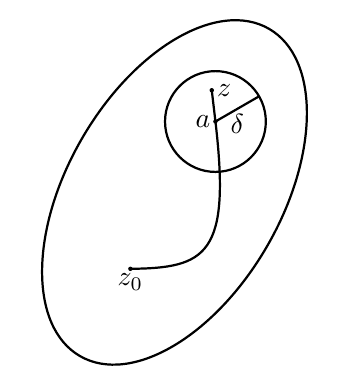
\begin{tikzpicture}[thick,every node/.style={inner sep=1.5pt},scale=0.8]
    \draw[rotate=60](0,0)ellipse(3 and 1.7);
    \draw(60:1.3)coordinate(a)node[left]{$a$}circle(0.8);
    \coordinate(z0)at(-1200:1.4);
    \draw(z0)node[below]{$z_0$}..controls(0.5,-1.2)and(0.9,-1)..(a)--
       ([turn]0:0.5)coordinate(z)node[right]{$z$};
    \foreach \x in{z0,z,a}
      \fill(\x)circle(1pt);
      \draw(a)--node[below]{$\delta$}++(30:0.8);
  \end{tikzpicture}
  \captionof{figure}{\label{fig3.6}}
\end{minipage}
  \begin{align*}
    \bigg|\frac{F(z)-F(a)}{z-a}-f(a)\bigg|
    & = \frac1{|z-a|}\bigg|F(z)-F(a)-f(a)(z-a)\bigg|\\
    & = \frac1{|z-a|}\bigg|\int_a^zf(\zeta)\dif \zeta-\int_a^zf(a)\dif \zeta\bigg|\\
    & = \frac1{|z-a|}\bigg|\int_a^z\big(f(\zeta)-f(a)\big)\dif \zeta\bigg|.
  \end{align*}
  由长大不等式,即知上式右端小于$\varepsilon$,这就证明了$F'(a)=f(a)$.
\end{proof}

作为定理 \ref{thm3.3.2} 的一个简单的推论,我们有
\begin{theorem}\label{thm3.3.3}
  设$D$是$\MC$中的单连通域,$f\in H(D)$,那么$F(z)=\int_{z_0}^zf(\zeta)\dif \zeta$是$f$在$D$中的一个原函数.
\end{theorem}
\begin{proof}
  在定理的假定下,由Cauchy积分定理知道,$f$沿$D$中任意可求长闭曲线的积分为零,由定理 \ref{thm3.3.2} 即得本定理.
\end{proof}

类似于微积分中的Newton--Leibniz公式,我们有
\begin{theorem}\label{thm3.3.4}
  设$D$是$\MC$中的单连通域,$f\in H(D),\varPhi$是$f$的任一原函数,那么
  \[
    \int_{z_0}^zf(\zeta)\dif \zeta = \varPhi(z)-\varPhi(z_0).
  \]
\end{theorem}
\begin{proof}
  证明方法也与微积分中一样.由定理 \ref{thm3.3.3} 知,由变上限积分确定的函数$F$是$f$的一个原函数,因而
  \[
    \big(\varPhi(z) - F(z)\big)' = f(z) - f(z) = 0.
  \]
  故由第 \ref{chap2} 章习题 \hyperlink{xiti2.2}{2.2} 的第 \hyperlink{xiti2.2.1}{1} 题知道$\varPhi(z)-F(z)$是一个常数,因而
  \begin{equation*}
    \int_{z_0}^zf(\zeta)\dif \zeta = F(z) - F(z_0) = \varPhi(z) - \varPhi(z_0). \qedhere
  \end{equation*}
\end{proof}

现在设$D$是多连通域,$f\in H(D)$,一般来说
  \[
    F(z) = \int_{z_0}^zf(\zeta)\dif \zeta
  \]
是一个多值函数,它在$z$点的值将随着连接$z_0$和$z$的曲线变化而变动.下面看一个具体的例子:

设$D=\MC\backslash\{0\}$,则$D$是一个二连通域,$f(z)=\frac1z$是$D$中的全纯函数,我们来研究积分
\[
  \int_1^z \frac1\zeta \dif \zeta.
\]
如果连接$1$和$z$的曲线$\gamma$不围绕原点(图 \ref{fig3.7}),那么$\frac1\zeta$沿$\gamma$的积分等于在实轴上从$1$到$|z|$的积分与圆弧$\gamma'$上的积分之和,即
\[
  \int\limits_\gamma\frac{\dif \zeta}{\zeta} = \int_1^{|z|} \frac{\dx}x+\int_0^{\arg z}\frac{\ii|z|\ee^{\ii\theta}}{|z|\ee^{\ii\theta}}\dif \theta = \log|z| + \ii\arg z = \log z.
\]
\begin{figure}[!ht]
  \centering
  \begin{minipage}[b]{0.48\linewidth}
    \centering
    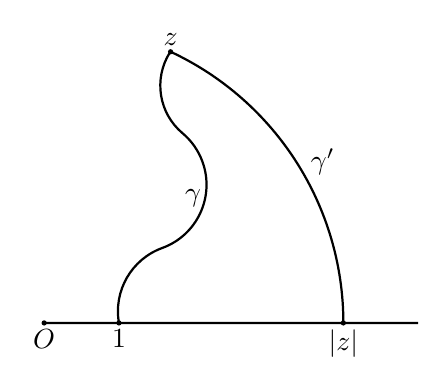
\begin{tikzpicture}[thick,every node/.style={inner sep=2pt},scale=0.95]
      \draw(0,0)node[below]{$O$}--(1,0)node[below]{$1$}--(4,0)node[below]{$|z|$}
        arc(0:65:4)coordinate(z) node[above]{$z$}(4,0)--(5,0);
      \foreach \x in{{0,0},{1,0},{4,0},z}
        \fill(\x)circle(1pt);
      \node at(30:4.3){$\gamma'$};
      \draw(1,0)arc(190:110:0.9)arc(-70:50:0.9)arc(-130:-212:0.83);
      \node at(40:2.6){$\gamma$};
    \end{tikzpicture}
    \caption{\label{fig3.7}}
  \end{minipage}\hfill
\begin{minipage}[b]{0.48\linewidth}
  \centering
  \begin{tikzpicture}[thick,every node/.style={inner sep=2pt},>={Stealth[width=4pt]}]
    \draw(0,0)coordinate(O)node[below left]{$O$};
    \fill(0,0)circle(1pt)(1,0)node[right]{$1$}circle(1pt);
    \draw(1,0)[bend right=5]to(40:1)coordinate(a)[bend right=35]to(95:1.2)
        coordinate(a1)[bend right=60]to(190:1.2)coordinate(b)
        [bend right=15]to(230:1)coordinate(b1)[bend right=60]to(0:0.3)
        [bend right=50]to(130:0.6)coordinate(d)[bend right=20]to(b)
        [bend right=40]to(-110:1.8)coordinate(b2)arc(-110:-30:0.7)coordinate(A)
        [bend right=18]to(a)[bend left=20]to(60:3)coordinate(z);
    \begin{scope}[very thin]
      \draw[->](1,0)[bend right=5]to(25:0.96);
      \draw[->](a)node[right]{$a$}[bend right=35]to(a1);
      \draw[->](b)node[left]{$b$}[bend right=15]to(230:1)node[below right,inner sep=3pt]{$c$};
      \draw[->](0:0.3)[bend right=50]to(130:0.6)node[above right,inner sep=3pt]{$d$};
      \draw[->](b)[bend right=40]to(-110:1.8)node[below right,inner sep=3pt]{$e$};
      \draw[->](A)[bend right=10]to(-20:0.764);
      \draw[->](a)[bend left=10]to(61.6:2.1);
    \end{scope}
    \fill(z)circle(1pt)node[right]{$z$};
  \end{tikzpicture}
  \caption{\label{fig3.8}}
\end{minipage}
\end{figure}

\noindent 如果连接$1$和$z$的曲线$\gamma$绕原点沿反时针方向转了$2$圈(图 \ref{fig3.8}),这时沿$\gamma$的积分可以分解为沿$\wideparen{1az}$,$\wideparen{abea}$和$\wideparen{bcdb}$的积分,即
\begin{equation}\label{eq3.3.1}
  \int\limits_\gamma\frac{\dif \zeta}{\zeta}
  = \int\limits_{\wideparen{1az}}\frac{\dif \zeta}{\zeta} + \int\limits_{\wideparen{abea}}\frac{\dif \zeta}{\zeta}+\int\limits_{\wideparen{bcdb}}\frac{\dif \zeta}{\zeta}.
\end{equation}
由于$\wideparen{abea}$和$\wideparen{bcdb}$是两条围绕原点的简单闭曲线,故由 \ref{sec3.2} 节的例 \ref{exam3.2.7},\eqref{eq3.3.1} 式右端的后两个积分都等于$2\pi\ii$.根据上面的计算,\eqref{eq3.3.1} 式右端的第一个积分为$\log z$,因而得
\[
  \int\limits_\gamma \frac{\dif \zeta}\zeta = \log z + 4\pi\ii.
\]
由此可见,随着绕原点圈数的不同,一般可得
\[
  \int\limits_\gamma\frac{\dif \zeta}\zeta = \log z+2k\pi\ii,k = 0,\pm1,\cdots,
\]
这恰好是对数函数$\Log z$.所以,对数函数也可用变上限的积分来定义.

\begin{xiti}
  \item 设$D$是域,$f,g\in H(D)$.如果$fg'$在$D$上有原函数$\varphi$. 证明:$f'g$在$D$上有原函数$fg-\varphi$.
  \item 设$D$是域,$f$是$D$上的连续函数. 如果$f$在$D$上有原函数,则对$D$中任意可求长简单闭曲线$\gamma$,均有$\int\limits_\gamma f(z)\dz=0$.
  \item 设$f\in C^n(\MC)\cap H(\MC)$,并且$f^{(n)}(z)\equiv0$. 证明: $f$必为次数不大于$n$的多项式.
  \item 设$\gamma$是从$0$到$1$且不经过$\pm\ii$的可求长曲线.证明:
    \[
      \int\limits_\gamma\frac{\dz}{1+z^2} = \frac\pi4 + k\pi,k = 0,\pm1,\pm2,\cdots.
    \]
  \item 设$f$是凸域$D$上的全纯函数,如果对每点$z\in D$,有$\Re \{f'(z)\}>0$,那么$f$是$D$上的单叶函数.
\end{xiti}

\section{Cauchy积分公式\label{sec3.4}}
Cauchy积分公式是Cauchy积分定理最重要的推论之一,它是全纯函数的一种积分表示,通过这种表示,我们可以证明全纯函数有任意阶导数,而且可以展开成幂级数.从它还可以推出全纯函数的其他一系列重要性质.
\begin{theorem}\label{thm3.4.1}
  设$D$是由可求长简单闭曲线$\gamma$围成的域,如果$f\in H(D)\cap C(\bar D)$,那么对任意$z\in D$,均有
  \begin{equation}\label{eq3.4.1}
    f(z) = \frac1{2\pi\ii}\int\limits_\gamma\frac{f(\zeta)}{\zeta-z}\dif \zeta.
  \end{equation}
\end{theorem}
\begin{proof}
  任取$z\in D$,因为$f$在$z$点连续,故对任意$\varepsilon>0$,存在$\delta>0$,使得当$|\zeta-z|<\delta$时,有$|f(\zeta)-f(z)|<\varepsilon$.今取$\rho<\delta$,使得$B(z,\rho)\subset D$.记$\gamma_\rho=\{\zeta:|\zeta-z|=\rho\}$,由$\gamma$和$\gamma_{\rho}$围成的二连通域记为$D'$(图 \ref{fig3.9}),则$\frac{f(\zeta)}{\zeta-z}$在$D'$中全纯,在$\bar {D'}$上连续.于是,由推论 \ref{cor3.2.6} 得

  \noindent\begin{minipage}{0.7\textwidth}
    \begin{equation}\label{eq3.4.2}
      \frac1{2\pi\ii}\int\limits_\gamma\frac{f(\zeta)}{\zeta-z}\dif \zeta
      = \frac1{2\pi\ii}\int\limits_{\gamma_\rho}\frac{f(\zeta)}{\zeta-z}\dif \zeta.
    \end{equation}
    又因为$\frac1{2\pi\ii}\int\limits_{\gamma_\rho}\frac{\dif \zeta}{\zeta-z}=1$,所以
    \begin{equation}\label{eq3.4.3}
      f(z) = \frac1{2\pi\ii}\int\limits_{\gamma_\rho}\frac{f(z)}{\zeta-z}\dif \zeta.
    \end{equation}
    于是,由 \eqref{eq3.4.2} 式、\eqref{eq3.4.3} 式及长大不等式即得
  \end{minipage}
  \begin{minipage}{0.3\textwidth}
    \centering
    \begin{tikzpicture}[thick,every node/.style={inner sep=2pt},>={Stealth[width=3pt]},scale=1.1]
      \draw[rotate=60](0,0)circle(2 and 1);
      \draw[rotate=60,->,thin](2,0)arc(0:310:2 and 1);
      \draw(60:0.6)circle(0.4);
      \fill(60:0.6)circle(1pt)node[right]{$z$};
      \draw(45:1.2)node{$\gamma_\rho$}(40:2)node{$\gamma$}(-120:1.3)node{$D'$};
      \draw[->,very thin]([xshift=0.4cm]60:0.6)--++(0,0.1);
    \end{tikzpicture}
    \captionof{figure}{\label{fig3.9}}
  \end{minipage}
  \begin{align*}
    \bigg|f(z)-\frac1{2\pi\ii}\int\limits_\gamma\frac{f(\zeta)}{\zeta-z}\dif \zeta\bigg|
    & = \bigg|\frac1{2\pi\ii}\int\limits_{\gamma_\rho}\frac{f(z)}{\zeta-z}\dif \zeta-\frac1{2\pi\ii}\int\limits_{\gamma_\rho}\frac{f(\zeta)}{\zeta-z}\dif \zeta\bigg|\\
    & = \frac1{2\pi}\bigg|\int\limits_{\gamma_\rho}\frac{f(z)-f(\zeta)}{\zeta-z}\dif \zeta\bigg|\le\frac1{2\pi}\cdot\frac{\varepsilon}\rho\cdot2\pi\rho\\
    & = \varepsilon.
  \end{align*}
  让$\varepsilon\to0$,即得所要证的等式 \eqref{eq3.4.1}.
\end{proof}

等式 \eqref{eq3.4.1} 称为\textbf{Cauchy积分公式}\index{G!公式!Cauchy积分公式},它表明全纯函数在域中的值由它在边界上的值所完全确定. \eqref{eq3.4.1} 式是全纯函数的一种积分表示,通过这种表示,我们可以证明全纯函数有任意阶导数,这实际上是下面更一般的结果的一个特殊情形:

设$\gamma$是$\MC$中一条可求长曲线(不一定是闭的),$g$是$\gamma$上的连续函数,如果$z\in\MC\backslash\gamma$,那么积分
\[
  \frac1{2\pi\ii}\int\limits_\gamma\frac{g(\zeta)}{\zeta-z}\dif \zeta
\]
是存在的,它定义了$\MC\backslash\gamma$上的一个函数$G(z)$,即
\[
  G(z) = \frac1{2\pi\ii}\int\limits_\gamma\frac{g(\zeta)}{\zeta-z}\dif \zeta,
\]
称它为\textbf{Cauchy型积分}\index{C!Cauchy型积分}.由Cauchy型积分确定的函数有很好的性质.
\begin{theorem}\label{thm3.4.2}
  设$\gamma$是$\MC$中的可求长曲线,$g$是$\gamma$上的连续函数,那么由Cauchy型积分确定的函数
  \[
    G(z) = \frac1{2\pi\ii}\int\limits_\gamma\frac{g(\zeta)}{\zeta-z}\dif \zeta,
  \]
 在$\MC\backslash\gamma$上有任意阶导数,而且
  \begin{equation}\label{eq3.4.4}
    G^{(n)}(z) = \frac{n!}{2\pi\ii}\int\limits_\gamma \frac{g(\zeta)}{(\zeta-z)^{n+1}}\dif \zeta,n=1,2,\cdots.
  \end{equation}
\end{theorem}
\begin{proof}
  我们用数学归纳法来证明等式 \eqref{eq3.4.4}.先设$n=1$,我们要证明
  \begin{equation}\label{eq3.4.5}
    G'(z) = \frac1{2\pi\ii}\int\limits_\gamma \frac{g(\zeta)}{(\zeta-z)^2}\dif \zeta,z\in\MC\backslash\gamma.
  \end{equation}
  任意取定$z_0\in\MC\backslash\gamma$,记$\rho=\inf_{\zeta\in\gamma}|\zeta-z_0|>0,\delta=\min\bigg\{1,\frac\rho2\bigg\}$,则当$\zeta\in\gamma,z\in B(z_0,\delta)$时,有$\bigg|\frac{z-z_0}{\zeta-z_0}\bigg|<\frac12$. 于是
  \begin{equation}\label{eq3.4.6}
    \frac1{\zeta-z} = \frac1{\zeta-z_0}\cdot\frac1{1-\frac{z-z_0}{\zeta-z_0}}
    = \frac1{\zeta-z_0}\bigg(1+\frac{z-z_0}{\zeta-z_0}+h(z,\zeta)\bigg),
  \end{equation}
  其中
  \begin{equation}\label{eq3.4.7}
    |h(z,\zeta)|\le\sum_{n=2}^\infty\bigg| \frac{z-z_0}{\zeta-z_0}\bigg|^n
    = \bigg|\frac{z-z_0}{\zeta-z_0}\bigg|^2\sum_{n=0}^\infty \bigg|\frac{z-z_0}{\zeta-z_0}\bigg|^n
    \le \frac2{\rho^2}|z-z_0|^2.
  \end{equation}
  这样,由 \eqref{eq3.4.6} 式便得
  \begin{align*}
    G(z) & = \frac1{2\pi\ii}\int\limits_\gamma\frac{g(\zeta)}{\zeta-z}\dif \zeta\\
    & = \frac1{2\pi\ii}\int\limits_\gamma\frac{g(\zeta)}{\zeta-z_0}\dif \zeta + \frac{z-z_0}{2\pi\ii}\int\limits_\gamma\frac{g(\zeta)}{(\zeta-z_0)^2}\dif \zeta
    + \frac1{2\pi\ii}\int\limits_\gamma\frac{g(\zeta)h(z,\zeta)}{\zeta-z_0}\dif \zeta,
  \end{align*}
  因而有
  \begin{equation}\label{eq3.4.8}
    \frac{G(z)-G(z_0)}{z-z_0} - \frac1{2\pi\ii}\int\limits_\gamma\frac{g(\zeta)}{(\zeta-z_0)^2}\dif \zeta = \frac1{2\pi\ii(z-z_0)}\int\limits_\gamma\frac{g(\zeta)h(z,\zeta)}{\zeta-z_0}\dif \zeta.
  \end{equation}
  若记$M=\sup_{\zeta\in\gamma}|g(\zeta)|$,由 \eqref{eq3.4.7} 式便知 \eqref{eq3.4.8} 式右端的绝对值不超过
  \[
    \frac{M|\gamma|}{\pi\rho^3|z-z_0|}\cdot|z-z_0|^2 = \frac{M|\gamma|}{\pi\rho^3}|z-z_0|.
  \]
  在 \eqref{eq3.4.8} 式两端令$z\to z_0$,即得
  \[
    G'(z) = \frac1{2\pi\ii}\int\limits_\gamma\frac{g(\zeta)}{(\zeta-z)^2}\dif \zeta.
  \]

  现设$n=k$时 \eqref{eq3.4.4} 式成立. 即
  \[
    G^{(k)}(z) = \frac{k!}{2\pi\ii}\int\limits_\gamma\frac{g(\zeta)}{(\zeta-z)^{k+1}}\dif \zeta,
  \]
  要证明
  \[
    G^{(k+1)}(z) = \frac{(k+1)!}{2\pi\ii}\int\limits_\gamma\frac{g(\zeta)}{(\zeta-z)^{k+2}}\dif \zeta.
  \]
  由 \eqref{eq3.4.6} 式和二项式定理,可得
  \begin{align*}
    \frac{1}{( \zeta -z) ^{k+1}} & = \frac{1}{( \zeta -z_0 ) ^{k+1}}\bigg( 1+\frac{z-z_0}{\zeta -z_0}+h( z,\zeta ) \bigg) ^{k+1}\\
    & = \frac{1}{( \zeta -z_0 ) ^{k+1}}\bigg( 1+(k+1)\frac{z-z_0}{\zeta -z_0}+H( z,\zeta ) \bigg) ^{k+1},
  \end{align*}
  由 \eqref{eq3.4.7} 式便得
  \begin{equation}\label{eq3.4.9}
    |H(z,\zeta)|\le C|z-z_0|^2,
  \end{equation}
  这里,$C$是一个常数. 于是
  \begin{align*}
    G^{(k)}(z) = {}& \frac{k!}{2\pi\ii}\int\limits_\gamma\frac{g(\zeta)}{(\zeta-z_0)^{k+1}}\dif \zeta\\
    & +\frac{(k+1)!}{2\pi\ii}(z-z_0)\int\limits_\gamma\frac{g(\zeta)}{(\zeta-z_0)^{k+2}}
    \dif \zeta+\frac{k!}{2\pi\ii}\int\limits_\gamma\frac{g(\zeta)H(z,\zeta)}{(\zeta-z_0)^{k+1}}
    \dif \zeta,
  \end{align*}
  即
  \begin{equation}\label{eq3.4.10}
    \begin{gathered}
      \frac{G^{( k )}( z ) -G^{( k )}( z_0 )}{z-z_0}-\frac{( k+1 ) !}{2\pi\ii}\int\limits_{\gamma}{\frac{g( \zeta )}{( \zeta -z_0 ) ^{k+2}}\text{d}\zeta}\\
      = \frac{k!}{2\pi\ii ( z-z_0 )}\int\limits_{\gamma}{\frac{g( \zeta ) H( z,\zeta )}{( \zeta -z_0 ) ^{k+1}}\text{d}\zeta}.
    \end{gathered}
  \end{equation}
  由 \eqref{eq3.4.9} 式便知 \eqref{eq3.4.10} 式右端的绝对值不超过$K|z-z_0|$,这里,$K$是一个常数. 在 \eqref{eq3.4.10} 式中令$z\to z_0$,即得
  \[
    G^{(k+1)}(z_0) = \frac{(k+1)!}{2\pi\ii}\int\limits_\gamma\frac{g(\zeta)}{(\zeta-z_0)^{k+2}}\dif \zeta.
  \]
  由于$z_0$是$D$中的任意点,归纳法证明完毕.
\end{proof}

这个定理实际上证明了在现在的情况下,微分运算和积分运算可以交换,公式很便于记忆.从定理 \ref{thm3.4.1} 和定理 \ref{thm3.4.2} 立刻可得
\begin{theorem}\label{thm3.4.3}
  设$D$是由可求长简单闭曲线$\gamma$围成的域,如果$f\in H(D)\cap C(\bar D)$,那么$f$在$D$上有任意阶导数,而且对任意$z\in D$,有
  \begin{equation*}
    f^{(n)}(z) = \frac{n!}{2\pi\ii}\int\limits_\gamma\frac{f(\zeta)}{(\zeta-z)^{n+1}}\dif \zeta,n=1,2,\cdots.
  \end{equation*}
\end{theorem}
\begin{proof}
  由定理 \ref{thm3.4.1},$f$可写为Cauchy型积分
  \[
    f(z) = \frac1{2\pi\ii}\int\limits_{\gamma}\frac{f(\zeta)}{\zeta-z}\dif \zeta.
  \]
  由于$f$在$\gamma$上连续,故由定理 \ref{thm3.4.2} 即得所要证的结果.
\end{proof}

\begin{theorem}\label{thm3.4.4}
  如果$f$是域$D$上的全纯函数,那么$f$在$D$上有任意阶导数.
\end{theorem}
\begin{proof}
  任取$z_0\in D$,取充分小的$\delta$,使得$\bar{B(z_0,\delta)}\subset D$.由定理 \ref{thm3.4.3},$f$在$B(z_0,\delta)$中有任意阶导数,又由于$z_0$是任意的,所以$f$在$D$中有任意阶导数.
\end{proof}

\begin{example}\label{exam3.4.5}
  计算积分
  \[
    \int\limits_{|z|=2} \frac{\dz}{z^2(z^2+16)}.
  \]
\end{example}
\begin{solution}
  令$f(z)=\frac1{z^2+16}$,则$f$在$\{z:|z|\le2\}$中全纯,根据定理 \ref{thm3.4.3},有
  \[
    \int\limits_{|z|=2}\frac{\dz}{z^2(z^2+16)}=2\pi\ii
    \bigg(\frac1{z^2+16}\bigg)'\bigg|_{z=0}=0.
  \]

  也可以这样计算:
  \[
    \int\limits_{|z|=2}\frac{\dz}{z^2(z^2+16)} = \frac1{16}
    \bigg\{\int\limits_{|z|=2}\frac{\dz}{z^2}-\int\limits_{|z|=2}\frac{\dz}{z^2+16}\bigg\} = 0.
  \]
  这是因为,由例 \ref{exam3.1.4},第一个积分为零;由Cauchy积分定理,第二个积分为零.
\end{solution}

类似于Cauchy积分定理,也有下面的
\begin{theorem}\label{thm3.4.6}
  设$\gamma_0,\gamma_1,\cdots,\gamma_k$是$k+1$条可求长简单闭曲线,$\gamma_1,\cdots,\gamma_k$都在$\gamma_0$的内部,$\gamma_1,\cdots,\gamma_k$中的每一条都在其他$k-1$条的外部,$D$是由这$k+1$条曲线围成的域,$D$的边界$\gamma$由$\gamma_0,\gamma_1,\cdots,\gamma_k$所组成.如果$f\in H(D)\cap C(\bar D)$,则对任意$z\in D$,有
  \[f(z)=\frac1{2\pi\ii}\int\limits_{\gamma}\frac{f(\zeta)}{\zeta-z}\dif \zeta.\]
  $f$在$D$内有任意阶导数,且
  \[
    f^{(n)}(z) = \frac{n!}{2\pi\ii}\int\limits_\gamma\frac{f(\zeta)}{(\zeta-z)^{n+1}}\dif \zeta,n=1,2,\cdots.
  \]
\end{theorem}

定理的证明和前面的一样,不再重复.
\begin{example}\label{exam3.4.7}
  计算积分
  \[
    \int\limits_{|z|=2} \frac{\dz}{(z^3-1)(z+4)^2}.
  \]
\end{example}
\begin{solution}
  作一个中心在原点、半径为$R$($R>4$)的大圆(图 \ref{fig3.10}),则在闭圆环
  \[
    \{z:2\le|z| \le R\}
  \]
  上,$f(z)=\frac1{z^3-1}$是全纯的. 于是,由定理 \ref{thm3.4.6} 得
  \begin{figure}[!ht]
    \centering
    \begin{tikzpicture}[thick,every node/.style={inner sep=2pt},>={Stealth[width=3pt]},scale=0.5]
      \draw(0,0)node[below]{$O$}--(2,0)node[below right]{$2$}--(5,0)node[right]{$R$};
      \draw(70:2)arc(70:433:2)node[above right]{$\gamma_2$};
      \draw[->](70:5)arc(70:433:5)node[above right]{$\gamma_1$};
      \fill(0,0)circle(2pt)(2,0)circle(2pt)(5,0)circle(2pt);
      \draw[->,very thin](70:2)--++(160:0.1);
    \end{tikzpicture}
    \caption{\label{fig3.10}}
  \end{figure}
  \[
    \int\limits_{\gamma_1}\frac{\dz}{(z^3-1)(z+4)^2}+
    \int\limits_{\gamma_2^-}\frac{\dz}{(z^3-1)(z+4)^2}=2\pi\ii\bigg(\frac1{z^3-1}\bigg)'
    \bigg|_{z=-4}=-\frac{32}{1323}\pi\ii,
  \]
  所以
  \begin{equation}\label{eq3.4.11}
    \int\limits_{|z|=2}\frac{\dz}{(z^3-1)(z+4)^2}
    = \frac{32\pi\ii}{1323}+\int\limits_{|z|=R}\frac{\dz}{(z^3-1)(z+4)^2}.
  \end{equation}
  由于当$|z|=R$时,有
  \[
    |(z^3-1)(z+4)^2| \ge (R^3-1)(R-4)^2,
  \]
  所以由长大不等式得
  \[
    \bigg|\int\limits_{|z|=R}\frac{\dz}{(z^3-1)(z+4)^2}\bigg|
    \le \frac{2\pi R}{(R^3-1)(R-4)^2}\to0\,\mbox{($R\to\infty$)}.
  \]
  故在 \eqref{eq3.4.11} 中令$R\to\infty$,即得
  \[
    \int\limits_{|z|=2}\frac{\dz}{(z^3-1)(z+4)^2}=\frac{32\pi\ii}{1323}. \qedhere
  \]
\end{solution}


\begin{xiti}
  \item 计算下列积分:
  \begin{enuma}
    \item $\int\limits_{|z-1|=1}\frac{\sin z}{z^2-1}\dz$;
    \item $\int\limits_{|z|=2}\frac{\dz}{1+z^2}$;
    \item $\int\limits_{4x^2+y^2=2y}\frac{\ee^{\pi z}}{(1+z^2)^2}\dz$;
    \item $\int\limits_{|z|=\frac32}\frac{\dz}{(z^2+1)(z^2+4)}$;
    \item $\int\limits_{|z|=2}\frac{\dz}{z^3(z-1)^3(z-3)^5}$;
    \item $\int\limits_{|z|=R}\frac{\dz}{(z-a)^n(z-b)}$,$n$为正整数,$a,b$不在圆周$|z|=R$上.
  \end{enuma}
  \item 设$\gamma$是可求长简单闭曲线,其内部为域$G_1$,外部为域$G_2$.如果$f\in H(G_2)\cap C(\bar G_2)$,而且
    \[
      \lim_{z\to\infty}f(z) = A,
    \]
    那么
    \[
      \frac1{2\pi\ii}\int\limits_\gamma\frac{f(\zeta)}{\zeta-z}\dif \zeta
      = \begin{cases}
      -f(z) + A, & z\in G_2;\\
      A, & z\in G_1,
      \end{cases}
    \]
    这里,$\gamma$关于$G_1$取正向. 通常,称它为\textbf{无界域的Cauchy积分公式}\index{G!公式!无界域的Cauchy积分公式}.
  \item 设$D$是由有限条可求长简单闭曲线围成的域,$z_1,\cdots,z_n$是$D$中$n$个彼此不同的点.如果$f\in H(D)\cap C(\bar D)$,证明:
    \[
      P(z) = \frac1{2\pi\ii}\int\limits_{\partial D}\frac{f(\zeta)}{\omega_n(\zeta)}
      \frac{\omega_n(\zeta)-\omega_n(z)}{\zeta-z}\dif \zeta
    \]
    是次数不超过$n-1$的多项式,并且
    \[
      P(z_k) = f(z_k), k=1,2,\cdots,n.
    \]
    其中,$\omega_n(z)=(z-z_1)\cdots(z-z_n)$.

    (\textbf{提示}:$\frac{\omega_n(\zeta)-\omega_n(z)}{\zeta-z}$是$z$的次数不超过$n-1$的多项式.)
  \item 称
    \[
      P_n(z) = \frac1{2^nn!}\frac{\dif ^n}{\dif z^n}(z^2-1)^n
    \]
    是\textbf{Legendre多项式}\index{L!Legendre多项式}. 证明:
    \begin{enuma}
      \item Legendre多项式有如下的积分表示:
        \[
          P_n(z)=\frac1{2\pi\ii}\int\limits_\gamma\frac{(\zeta^2-1)^n}{2^n(\zeta-z)^{n+1}}
          \dif \zeta,
        \]
        其中,$\gamma$是任意内部包含$z$的可求长简单闭曲线;
      \item 如果取
        \[
          \gamma = \left\{\zeta\in\MC:|\zeta-x|=\sqrt{x^2-1}\right\}\; \mbox{($1<x<\infty$)},
        \]
        那么有如下的\textbf{Laplace公式}\index{G!公式!Laplace公式}:
        \[
          P_n(x) = \frac1\pi\int_0^\pi\big(x+\sqrt{x^2-1} \cos\theta\big)^n\dif \theta.
        \]
    \end{enuma}
  \item 设$f\in H\big(B(0,1)\big)\cap C\big(\bar{B(0,1)}\big)$. 证明:
    \begin{enuma}
      \item $\frac2\pi\int_0^{2\pi}f(\ee^{\ii\theta})\cos^2\bigg(\frac\theta2\bigg)\dif \theta=2f(0)+f'(0)$;
      \item $\frac2\pi\int_0^{2\pi}f(\ee^{\ii\theta})\sin^2\bigg(\frac\theta2\bigg)\dif \theta=2f(0)-f'(0)$.
    \end{enuma}

    (\textbf{提示}:分别计算积分
    \[
      \frac1{2\pi\ii}\int\limits_{|\zeta|=1}\bigg(2+\zeta+\frac1\zeta\bigg)f(\zeta)
      \frac{\dif \zeta}\zeta
    \]
    和
    \[
      \frac1{2\pi\ii}\int\limits_{|\zeta|=1}\bigg(2-\zeta-\frac1\zeta\bigg)f(\zeta)
     \frac{\dif \zeta}\zeta
     \]
     即可.)
  \item 利用上题结果证明:设$f\in H\big(B(0,1)\big)\cap C\big(\bar{B(0,1)}\big)$,且$f(0)=1,\Re f(z)\ge0$,那么
    \[
      -2\le\Re f'(0) \le 2.
    \]
  \item 设$f$在角状域$G=\bigg\{z\in\MC:0<\arg z<\frac\pi4\bigg\}$中全纯,在$\bar G$上连续.如果$f$在正实轴的区间$[a,b]$上等于零,证明:$f$在$G$中恒等于零.
  \item (\textbf{Schwarz积分公式}\index{G!公式!Schwarz积分公式})设$f\in H\big(B(0,R)\big)\cap C\big(\bar{B(0,R)}\big)$,$f=u+\ii v$. 证明:$f$可用实部表示为
      \[
        f(z) = \frac1{2\pi}\int_0^{2\pi}\frac{R\ee^{\ii\theta}+z}{R\ee^{\ii\theta}-z}
        u(R\ee^{\ii\theta})\dif \theta+\ii v(0).
      \]
  \item 设$f\in H\big(B(0,R)\big)\cap C\big(\bar{B(0,R)}\big)$,$f=u+\ii v$,则对任意$0<r\le R$,有
    \[
      f'(0) = \frac1{\pi r}\int_0^{2\pi}u(r\ee^{\ii\theta})\ee^{-\ii\theta}\dif \theta.
    \]
\end{xiti}

\section{Cauchy积分公式的一些重要推论\label{sec3.5}}
前面我们已经从Cauchy积分公式出发,证明了全纯函数有任意阶导数,并且得到了这些导数的积分表示,从这些表示又可得到全纯函数的另外一些重要性质.
\begin{theorem}[(\textbf{Cauchy不等式})]\label{thm3.5.1}\index{D!定理!Cauchy不等式}
  设$f$在$B(a,R)$中全纯,且对任意$z\in B(a,R)$,有$|f(z)|\le M$,那么
\begin{equation}\label{eq3.5.1}
  |f^{(n)}(a)|\le\frac{n!M}{R^n}, n=1,2,\cdots.
\end{equation}
\end{theorem}
\begin{proof}
  取$0<r<R$,则$f$在闭圆盘$\bar{B(a,r)}$中全纯,由定理 \ref{thm3.4.3},得
\begin{equation*}
  f^{(n)}(a)=\frac{n!}{2\pi\ii}\int\limits_{|\zeta-a|=r}\frac{f(\zeta)}{(\zeta-a)^{n+1}}\dif \zeta,n=1,2,\cdots.
\end{equation*}
于是,由长大不等式得
\[
  |f^{(n)}(a)|\le\frac{n!}{2\pi} \cdot \frac M{r^{n+1}}\cdot2\pi r = \frac{n!M}{r^n}.
\]
让$r\to R$,即得所要证的不等式 \eqref{eq3.5.1}.
\end{proof}


这个不等式给出了圆盘上全纯函数的各阶导数在圆心处值的估计,利用这个估计可以证明下面的
\begin{theorem}[(\textbf{Liouville})]\label{thm3.5.2}\index{D!定理!Liouville定理}
  有界整函数必为常数.
\end{theorem}
\begin{proof}
  设$f$为一有界整函数,其模的上界设为$M$,即对任意$z\in\MC$,有$|f(z)|\le M$.任取$a\in\MC$,以$a$为中心、$R$为半径作圆,因为$f$为整函数,故由Cauchy不等式可得
  \[
    |f'(a)| \le \frac MR.
  \]
  这个不等式对任意$R>0$都成立,让$R\to\infty$,即得$f'(a)=0$.因为$a$是任意的,所以在全平面上有$f'(z)\equiv0$,因而$f$是常数.
\end{proof}

从Liouville定理立刻可得
\begin{theorem}[(\textbf{代数学基本定理})]\label{thm3.5.3}\index{D!定理!代数学基本定理}
  任意复系数多项式
  \[
    P(z) = a_0z^n + a_1z^{n-1} + \cdots + a_n,a_0\ne0
  \]
  在$\MC$中必有零点.
\end{theorem}
\begin{proof}
  如果$P(z)$在$\MC$中没有零点,那么$f(z)=\frac1{P(z)}$是一个整函数.由于$\lim_{z\to\infty}P(z)=\infty$,故当$|z|>R$时,$|f(z)|\le1$;而当$|z|\le R$时,$f$是有界的,因而$f$是一有界整函数. 由Liouville定理,$f$应是一常数.这个矛盾证明了$P$在$\MC$中必有零点.
\end{proof}

考虑到实系数多项式在实数域中未必有零点,这个定理给出了复数域的又一重要性质.

从定理 \ref{thm3.4.4} 还可得到Cauchy定理的逆定理:
\begin{theorem}[(\textbf{Morera})]\label{thm3.5.4}\index{D!定理!Morera定理}
  如果$f$是域$D$上的连续函数,且沿$D$内任一可求长闭曲线的积分为零,那么$f$在$D$上全纯.
\end{theorem}
\begin{proof}
  由定理 \ref{thm3.3.2},存在$F\in H(D)$,使得$F'(z)=f(z)$在$D$中成立.由定理 \ref{thm3.4.4},$F$是$D$中的全纯函数,所以$f$也是全纯函数.
\end{proof}
\begin{xiti}
  \item 设$f$是有界整函数,$z_1,z_2$是$B(0,r)$中任意两点.证明:
    \[
      \int\limits_{|z|=r} \frac{f(z)}{(z-z_1)(z-z_2)}\dz = 0.
    \]
    并由此得出Liouville定理.
  \item 设$f$是整函数,如果当$z\to\infty$时,$f(z)=O(|z|^\alpha),\alpha\ge0$,证明$f$是次数不超过$[\alpha]$的多项式.
  \item 设$f$是域$D$上的连续函数,如果对于任意边界和内部都位于$D$中的三角形域$\varDelta$,总有$\int\limits_{\partial D}f(z)\dz=0$,那么$f$是$D$上的全纯函数.
  \item 设$f$是整函数,如果
    \[
      f(\MC)\subset\{z\in\MC:\Im z>0\},
    \]
    证明$f$是一个常值函数.
  \item 设$f$是整函数,如果
    \[
      f(\MC)\subset \MC\backslash[0,1],
    \]
    证明$f$是一个常值函数.
  \item 设$f$在域$D$上全纯,$z_0\in D$,定义
    \[
      F(z) = \begin{cases}
        \frac{f(z)-f(z_0)}{z-z_0}, & z\in D\backslash\{z_0\};\\
        f'(z_0), & z = z_0.
      \end{cases}
    \]
    证明:$F\in H(D)$.
  \item 设$\gamma$是可求长曲线,$f$在域$D$上连续,在$D\backslash\gamma$上全纯.证明:$f$在$D$上全纯.
  \item 设$f$是域$D$上的连续函数,如果对于任意边界和内部都位于$D$中的弓形域$G$,总有$\int\limits_{\partial G}f(z)\dz=0$,那么$f$是$D$上的全纯函数.如果把弓形域换成圆盘,结论是否仍然成立?
\end{xiti}

\section{非齐次Cauchy积分公式\label{sec3.6}}
设$f=u+\ii v$,如果$u,v$作为$x,y$的二元函数是可微的,而且$u,v$满足Cauchy--Riemann方程,那么$f$就是全纯函数.我们已经看到,全纯函数有一系列良好的性质.这一节中,我们只假定$u,v$具有一阶连续偏导数,但不一定满足Cauchy--Riemann方程,这就是第 \ref{chap2} 章 \ref{sec2.2} 节中提到的$C^1$函数类.我们要把Cauchy积分公式推广到这一函数类,用到的工具主要是微积分中的Green公式,但要把它写成复变数的形式.

把$z,\bar z$看成独立变量,定义微分$\dz,\dzz$的外积为
\begin{align*}
  & \dz\wedge \dz = 0,\\
  & \dzz\wedge \dzz = 0,\\
  & \dz\wedge \dzz = -\dzz\wedge \dz.
\end{align*}
由于$\dz=\dx+\ii\dy,\dzz=\dx-\ii\dy$,所以
\begin{align*}
  \dz\wedge\dzz & = (\dx+\ii\dy)\wedge(\dx-\ii\dy)\\
  & = \ii\dy\wedge\dx-\ii\dx\wedge\dy\\
  & = -2\ii\dx\wedge\dy = -2\ii\dif A.
\end{align*}
这里,$\dif A$是面积元素;$\dx,\dy$的外积定义与$\dz,\dzz$的外积定义一样,即$\dx\wedge\dx=0,\dy\wedge\dy=0,\dx\wedge\dy=-\dy\wedge\dx$.

称$z,\bar z$的函数$f(z,\bar z)$为\textbf{零次微分形式}\index{W!微分形式!零次微分形式},$f_1(z,\bar z)\dz+f_2(z,\bar z)\dzz$为\textbf{一次微分形式}\index{W!微分形式!一次微分形式},$f(z,\bar z)\dz\wedge\dzz$为\textbf{二次微分形式}\index{W!微分形式!二次微分形式}.定义算子$\partial,\bar\partial$如下:
\begin{align*}
  & \partial f = \pp fz\dz,\\
  & \bar \partial f = \pp f{\bar z}\dzz,
\end{align*}
这里,$\pp{}z,\pp{}{\bar z}$由第 \ref{chap2} 章 \ref{sec2.2} 节中的 \eqref{eq2.2.3} 式定义. 定义算子$\dif =\partial+\bar\partial$,即
\begin{equation}\label{eq3.6.1}
  \dif f = \partial f + \bar\partial f = \pp fz\dz + \pp f{\bar z}\dzz.
\end{equation}
算子$\partial,\bar\partial$对一次微分形式的作用定义为
\begin{align*}
  \partial\big(f_1(z,\bar z)\dz+f_2(z,\bar z)\dzz\big)
  & = \pp{f_1}z\dz \wedge \dz + \pp{f_2}z \d z\wedge\dzz = \pp{f_2}z\dz \wedge \dzz,\\
  \bar\partial\big(f_1(z,\bar z)\dz+f_2(z,\bar z)\dzz\big)
  & = \pp{f_1}{\bar z}\dzz\wedge\dz+\pp{f_2}{\bar z}\dzz\wedge\dzz=-\pp{f_1}{\bar z}\dz\wedge\dzz,
\end{align*}
所以
\begin{equation}\label{eq3.6.2}
  \dif \big(f_1(z,\bar z)\dz + f_2(z,\bar z)\dzz\big)
  = \bigg(\pp{f_2}z-\pp{f_1}{\bar z}\bigg)\dz\wedge\dzz.
\end{equation}
$\partial,\bar\partial$作用在二次微分形式上的结果都是零:
\begin{align*}
  & \partial\big(f(z,\bar z)\dz\wedge\dzz\big) = \pp fz\dz\wedge\dz\wedge\dzz = 0,\\
  & \bar\partial\big(f(z,\bar z)\dz\wedge\dzz\big) = \pp fz\dzz\wedge\dz\wedge\dzz = 0,
\end{align*}
因而
\begin{equation}\label{eq3.6.3}
  \dif \big(f(z,\bar z)\dz\wedge\dzz\big)=0.
\end{equation}

定义$\dif ^2\omega=\dif (\dif \omega)$. 当$\omega$是一$C^2$函数时,由 \eqref{eq3.6.1} 式和 \eqref{eq3.6.2} 式,得
\begin{equation}\label{eq3.6.4}
  \dif ^2\omega=\dif (\dif \omega) = \dif \bigg(
  \pp\omega z\dz+\pp\omega{\bar z}\dzz\bigg) = \bigg(\pppp\omega z{\bar z}-
  \pppp\omega{\bar z}z\bigg)\dz\wedge\dzz=0.
\end{equation}
当$\omega$是一个一次微分形式时,由 \eqref{eq3.6.2} 式知$\dif \omega$是一个二次微分形式,由 \eqref{eq3.6.3} 式即知$\dif ^2\omega=0$.当$\omega$是一个二次微分形式时,由 \eqref{eq3.6.3} 式知$\dif ^2\omega=0$.总之,不论$\omega$是零次、一次或二次微分形式,都有$\dif ^2\omega=0$,所以$\dif ^2=0$.

定义$\partial^2\omega=\partial(\partial\omega),\bar\partial^2\omega=
\bar\partial(\bar\partial\omega),\partial\bar\partial\omega=\partial(\bar\partial\omega),
\bar\partial\partial\omega=\bar\partial(\partial\omega)$. 同样可以证明
\begin{equation}\label{eq3.6.5}
  \begin{aligned}
    & \partial^2 = 0,\\
    & \bar\partial^2 = 0,\\
    & \bar\partial\partial + \partial\bar\partial = 0.
  \end{aligned}
\end{equation}

现在证明复变数形式的\textbf{Green公式}:\index{G!公式!Green公式}
\begin{theorem}\label{thm3.6.1}
  设$D$和$\partial D$如定理 \ref{thm3.2.5} 中所述,如果$\omega=f_1(z,\bar z)\dz+f_2(z,\bar z)\dzz$是域$D$上的一个一次微分形式,这里,$f_1,f_2\in C^1(\bar D)$,那么
\begin{equation}\label{eq3.6.6}
  \int\limits_{\partial D}\omega = \int\limits_D\dif \omega.
\end{equation}
\end{theorem}
\begin{proof}
  记$f_1=u_1+\ii v_1,f_2=u_2+\ii v_2$,这里,$u_1,v_1,u_2,v_2$是$z,\bar z$的实值函数,于是
  \begin{equation}\label{eq3.6.7}
    \begin{aligned}
      \omega & = f_1\dz + f_2\dzz\\
      & = (u_1+\ii v_1)(\dx+\ii\dy)+(u_2+\ii v_2)(\dx-\ii\dy)\\
      & = \{(u_1+u_2)\dx+(-v_1+v_2)\dy\}+\ii\{(v_1+v_2)\dx+(u_1-u_2)\dy\}.
    \end{aligned}
  \end{equation}
  由 \eqref{eq3.6.2} 式得
  \begin{equation}\label{eq3.6.8}
    \begin{aligned}
      \dif \omega & = \bigg(\pp{f_2}z-\pp{f_1}{\bar z}\bigg)\dz\wedge\dzz\\
      & = -\bigg\{\frac12\bigg(\pp{}x-\ii\pp{}y\bigg)(u_2+\ii v_2)
      -\frac12\bigg(\pp{}x+\ii\pp{}y\bigg)(u_1+\ii v_1)\bigg\}2\ii\dif A\\
      & = \bigg\{\bigg(\pp{v_2}x-\pp{v_1}x-\pp{u_2}y-\pp{u_1}y\bigg)
      + \ii\bigg(\pp{u_1}x-\pp{u_2}x-\pp{v_1}y-\pp{v_2}y\bigg)\bigg\}\dif A.
    \end{aligned}
  \end{equation}
  根据Green公式,我们有
  \begin{align}
    & \int\limits_{\partial D}(u_1+u_2)\dx+(-v_1+v_2)\dy
    = \int\limits_D\bigg\{\pp{}x(-v_1+v_2)-\pp{}y(u_1+u_2)\bigg\}\dif A,\label{eq3.6.9}\\
    & \int\limits_{\partial D}(v_1+v_2)\dx+(u_1-u_2)\dy
    = \int\limits_D\bigg\{\pp{}x(u_1-u_2)-\pp{}y(v_1+v_2)\bigg\}\dif A.\label{eq3.6.10}
  \end{align}
  由等式 \eqref{eq3.6.7},\eqref{eq3.6.8},\eqref{eq3.6.9},\eqref{eq3.6.10} 即得我们要证明的公式 \eqref{eq3.6.6}.
\end{proof}

公式 \eqref{eq3.6.6} 在高维空间中也成立,通常称为\textbf{Stokes公式},\index{G!公式!Stokes公式}这里只是它的一个特例.下面,我们就用它来证明$C^1$函数的Cauchy积分公式:
\begin{theorem}\label{thm3.6.2}
  设$D$和$\partial D$如定理 \ref{thm3.2.5} 中所述,如果$f\in C^1(\bar D)$,那么对任意$z\in D$,有
  \begin{equation}\label{eq3.6.11}
    f(z) = \frac1{2\pi\ii}\int\limits_{\partial D}\frac{f(\zeta)}{\zeta-z}\dif \zeta
    + \frac1{2\pi\ii}\int\limits_D\pp{f(\zeta)}{\bar\zeta}\frac1{\zeta-z}\dif \zeta\wedge\dif \bar\zeta.
  \end{equation}
\end{theorem}
\begin{proof}
  不妨设$D$是图 \ref{fig3.11} 所示的二连通域,$D$的边界$\partial D$由$\gamma_0$和$\gamma_1$组成.任取$z\in D$,因为$f$在$z$点连续,故对任意$\varepsilon>0$,存在$\delta>0$,当$|\zeta-z|<\delta$时,$|f(\zeta)-f(z)|<\varepsilon$. 记$\rho=\inf_{\zeta\in\partial D}|\zeta-z|>0$,取$\eta$,使得$0<\eta<\min\{\rho,\delta\}$,于是$\bar{B(z,\eta)}\subset D$. 记$B_\eta=B(z,\eta)$,令$G_\eta=D\backslash\bar B_\eta$,则$G_\eta$的边界$\partial G_\eta$由$\gamma_0,\gamma_1$和$\partial B_\eta$三条曲线组成. 考虑一次形式
  \[
    \omega = \frac{f(\zeta)}{\zeta-z}\dif \zeta,
  \]
  它在域$G_\eta$上满足定理 \ref{thm3.6.1} 的条件,因而有
  \begin{equation}\label{eq3.6.12}
    \int\limits_{\partial G_\eta}\omega = \int\limits_{G_\eta}\dif \omega.
  \end{equation}
  \begin{minipage}{0.7\textwidth}
    由于$\frac1{\zeta-z}$在$G_\eta$中全纯,所以
    \begin{align*}
      \bar\partial \omega&=\pp{}{\bar\zeta}\bigg(\frac{f(\zeta)}{\zeta-z}\bigg)\dif \bar\zeta\wedge\dif \zeta\\
      & = \bigg\{f(\zeta)\pp{}{\bar\zeta}\bigg(\frac1{\zeta-z}\bigg)
      + \pp{f(\zeta)}{\bar\zeta}\frac1{\zeta-z}\bigg\}\dif \bar\zeta\wedge\dif \zeta\\
      & = \pp{f(\zeta)}{\bar\zeta}\frac1{\zeta-z}\dif \bar\zeta\wedge\dif \zeta.
    \end{align*}
    易知
    \[
     \partial\omega = \pp{}\zeta\bigg(\frac{f(\zeta)}{\zeta-z}\bigg)\dif \zeta\wedge\dif \zeta,
    \]
  \end{minipage}
  \begin{minipage}{0.3\textwidth}
    \centering
    \begin{tikzpicture}[thick,every node/.style={inner sep=2pt},>={Stealth[width=3pt]}]
      \begin{scope}[rotate=70]
        \draw(0,0)circle(3 and 1.5);
        \draw[->,very thin](0,-1.5)arc(-90:-40:3 and 1.5);
        \draw[->,very thin](3,0)arc(0:70:3 and 1.5);
        \draw(1.5,0)circle(0.3);\fill(1.5,0)circle(1pt)(-1.9,0)circle(1pt);
        \filldraw[xshift=-1.9cm,pattern=north east lines,draw=black](0,0)circle(0.5);
        \draw[xshift=-1.9cm,->](240:0.5)--++(150:0.12);
      \end{scope}
      \draw(64:1.5)node{$z$}(57:2)node{$\partial B_\eta$}(-88:1.9)node{$\gamma_1$}
         (1.7,-0.4)node{$\gamma_0$};
    \end{tikzpicture}
    \captionof{figure}{\label{fig3.11}}
  \end{minipage}\\
  因而
  \[
    \dif \omega = \partial\omega+\bar\partial\omega = \pp{f(\zeta)}{\bar\zeta}\frac1{\zeta-z}
    \dif \bar\zeta\wedge\dif \zeta.
  \]
  这样,\eqref{eq3.6.12} 式可以写成
  \begin{equation}\label{eq3.6.13}
    \int\limits_{\partial D}\frac{f(\zeta)}{\zeta-z}\dif \zeta
    -\int\limits_{\partial B_\eta}\frac{f(\zeta)}{\zeta-z}\dif \zeta
    = \int\limits_{G_\eta}\pp{f(\zeta)}{\bar\zeta}\frac1{\zeta-z}\dif \bar\zeta\wedge
    \dif \zeta.
  \end{equation}
  注意
  \begin{align*}
    \int\limits_{\partial B_\eta}\frac{f(\zeta)}{\zeta-z}\dif \zeta
    & = \int\limits_{\partial B_\eta}\frac{f(\zeta)-f(z)}{\zeta-z}\dif \zeta
    + f(z)\int\limits_{\partial B_\eta}\frac{\dif \zeta}{\zeta-z}\\
    & = \int\limits_{\partial B_\eta}\frac{f(\zeta)-f(z)}{\zeta-z}\dif \zeta+2\pi\ii f(z),
  \end{align*}
  而
  \[
    \bigg|\int\limits_{\partial B_\eta}\frac{f(\zeta)-f(z)}{\zeta-z}\dif \zeta\bigg|\le\int\limits_{\partial B_\eta}\frac{|f(\zeta)-f(z)|}{|\zeta-z|}
    |\dif \zeta|\le\frac{\varepsilon}{\eta}\cdot2\pi\eta = 2\pi\varepsilon,
  \]
  由此即得
  \begin{equation}\label{eq3.6.14}
    \lim_{\eta\to0}\int\limits_{\partial B_\eta}\frac{f(\zeta)}{\zeta-z}\dif \zeta
    = 2\pi\ii f(z).
  \end{equation}
  另一方面,由于$\pp f{\bar \zeta}$在$\bar B_\eta$上连续,故有常数$M$,使得$\bigg|\pp f{\bar \zeta}\bigg|\le M$在$\bar B_\eta$上成立.于是
  \[
    \bigg|\int\limits_{B_\eta}\pp f{\bar\zeta}\frac1{\zeta-z}\dif \bar\zeta\wedge\dif \zeta\bigg|\le2\int\limits_{B_\eta}\bigg|\pp f{\bar\zeta}\bigg|\frac1{|\zeta-z|}\dif A\le 4M\pi\eta\to0\;\mbox{($\eta\to0$)}.
  \]
  因而
  \begin{equation}\label{eq3.6.15}
    \begin{aligned}
      \lim_{\eta\to0}\int\limits_{G_\eta}\pp f{\bar\zeta}\frac1{\zeta-z}\dif \bar\zeta\wedge\dif \zeta & = \lim_{\eta\to0}\bigg\{
      \int\limits_{D}\pp f{\bar\zeta}\frac1{\zeta-z}\dif \bar\zeta\wedge\dif \zeta-\int\limits_{B_\eta}\pp f{\bar\zeta}\frac1{\zeta-z}\dif \bar\zeta\wedge\dif \zeta\bigg\}\\
      & = \int\limits_D\pp f{\bar\zeta}\frac1{\zeta-z}\dif \bar\zeta\wedge\dif \zeta.
    \end{aligned}
  \end{equation}
  在等式 \eqref{eq3.6.13} 两端令$\eta\to0$,并利用 \eqref{eq3.6.14} 式和 \eqref{eq3.6.15} 式,即得所要证明的公式 \eqref{eq3.6.11}.
\end{proof}

如果$f\in H(D)$,那么由Cauchy--Riemann方程,$\pp f{\bar \zeta}=0$,这时公式 \eqref{eq3.6.11} 右端的第二项就消失了,公式 \eqref{eq3.6.11} 就是Cauchy积分公式.所以,公式 \eqref{eq3.6.11} 是Cauchy积分公式在$C^1$函数类中的推广,有时也称为\textbf{非齐次Cauchy积分公式}\index{G!公式!非齐次Cauchy积分公式}.

公式 \eqref{eq3.6.11} 首先是由Pompeiu在1912年证明的(所以有时也称之为\textbf{Pompeiu公式}\index{G!公式!Pompeiu公式}),但长期以来似乎被人们遗忘了.直到1950年,Grothendieck和Dolbeault用它来解$\bar\partial$方程时,人们才发现它的意义所在.这就是我们在下一节中要讨论的内容.
\begin{xiti}
  \item 设$D$是由有限条可求长简单闭曲线围成的域,$f\in C^1(\bar D)$.证明:
    \begin{enuma}
      \item $\iint\limits_D\pp{f(\zeta)}{\bar\zeta}\dif \bar\zeta\wedge\dif \zeta=\int\limits_{\partial D}f(\zeta)\dif \zeta$;
      \item $\iint\limits_D\pp{f(\zeta)}{\zeta}\dif \zeta\wedge\dif \bar\zeta=\int\limits_{\partial D}f(\zeta)\dif \bar\zeta$.
    \end{enuma}
  \item 设$D$是由有限条可求长简单闭曲线围成的域,$f,g\in C^1(\bar D)$. 证明(\textbf{Green公式}\index{G!公式!Green公式}):
    \[
      \iint\limits_D\bigg(\pp{g(\zeta)}\zeta-\pp{f(\zeta)}{\bar\zeta}\bigg)
      \dif \zeta\wedge\dif \bar\zeta=\int\limits_{\partial D}
      \big(f(\zeta)\dif \zeta+g(\zeta)\dif \bar\zeta\big).
    \]
  \item 设$D$是由有限条光滑简单闭曲线围成的域,$\boldsymbol n$是$\partial D$的单位法向量场,指向$D$的外部,$u,v\in C^2(\bar D)$. 证明:
    \begin{enuma}
      \item $\iint\limits_Du(z)\Delta v(z)\dx\dy+\iint\limits_D\bigg(
        \pp{u(z)}x\pp{v(z)}x+\pp{u(z)}y\pp{v(z)}y\bigg)\dx\dy=\int\limits_{\partial D}
        u(z)\pp{v(z)}{\boldsymbol n}|\dz|$;
      \item $\iint\limits_D\big(u(z)\Delta v(z)-v(z)\Delta u(z)\big)\dx\dy
        =\iint\limits_{\partial D}\bigg(u(z)\pp{v(z)}{\boldsymbol n}
        -v(z)\pp{u(z)}{\boldsymbol n}\bigg)|\dz|$.
    \end{enuma}
  \item 设$D$是由有限条可求长简单闭曲线围成的域,$f$在$\bar D$上全纯,$z\in D$. 证明:
    \[
      \iint\limits_D\frac{f'(\zeta)}{\bar\zeta-\bar z}\dif \zeta\wedge\dif \bar\zeta
      = \int\limits_{\partial D}\bigg(\frac{f(\zeta)}{\zeta-z}\dif \zeta+\frac{f(\zeta)}{\bar \zeta-\bar z}\dif \bar\zeta\bigg).
    \]
\end{xiti}

\section{一维 \texorpdfstring{$\bar \partial$}{∂̅}问题的解}
所谓一维$\bar\partial$问题,是指在域$D$上给定一个函数$f$,要求函数$u$,使得在$D$上有
\[
  \pp{u(z)}{\bar z} = f(z),z\in D.
\]
$u$就称为$\bar\partial$问题的解. \ref{sec3.6} 节介绍的非齐次Cauchy积分公式可以用来构造$\bar\partial$问题的解.为此需要一个引理,这个引理在讨论其他问题时也很有用.
\begin{definition}\label{def3.7.1}
  设$\varphi$是$\MC$上的函数,使$\varphi$不取零值的点集的闭包称为$\varphi$的\textbf{支集},\index{Z!支集}记为$\supp\varphi$,即
  \[
    \supp\varphi = \bar{\{z\in\MC:\varphi(z)\ne0\}}.
  \]
\end{definition}
\begin{lemma}\label{lemma3.7.2}
  设$a$是$\MC$中任意一点,$0<r<R$,则必存在$\varphi$,满足下列条件:
  \begin{eenum}
    \item $\varphi\in C^{\infty}(\MC)$;
    \item $\supp\varphi\subset B(a,R)$;
    \item 当$z\in\bar{B(a,r)}$时,$\varphi(z)\equiv1$;
    \item 对于任意$z\in\MC,0\le\varphi(z)\le1$.
  \end{eenum}
\end{lemma}
\begin{proof}
  令$r<R_1<R$和
  \begin{align*}
    & h_1(z) = \left\{\begin{aligned}
    & \ee^{\frac1{|z-a|^2-R_1^2}}, & & z\in B(a,R_1);\\
    & 0,& & z\notin B(a,R_1),
      \end{aligned}\right.\\
    & h_2(z) = \left\{\begin{aligned}
    & 0,& & z\in \bar{B(a,r)};\\
    & \ee^{\frac1{r^2-|z-a|^2}}, & & z\notin\bar{B(a,r)},
    \end{aligned}\right.
  \end{align*}
  那么$h_1,h_2\in C^\infty(\MC)$. 又令
  \[
    \varphi(z) = \frac{h_1(z)}{h_1(z)+h_2(z)},
  \]
  则$\varphi\in C^\infty(\MC)$. 而且当$z\in \bar{B(a,r)}$时,$\varphi(z)\equiv1$;当$z\notin B(a,R_1)$时,$\varphi(z)\equiv0$,即$\supp\varphi\subset B(a,R)$.对于任意$z\in\MC,0\le\varphi(z)\le1$显然成立. $\varphi$即为所求的函数.
\end{proof}

现在可以证明
\begin{theorem}\label{thm3.7.3}
  设$D$是$\MC$中的域,$f\in C^1(D)$.令
  \begin{equation}\label{eq3.7.1}
    u(z) = \frac1{2\pi\ii}\int\limits_D\frac{f(\zeta)}{\zeta-z}\dif \zeta\wedge\dif \bar \zeta,z\in D,
  \end{equation}
  则$u\in C^1(D)$,且对任意$z\in D$,有$\pp{u(z)}{\bar z}=f(z)$.
\end{theorem}
\begin{proof}
  把$f$的定义扩充到整个复平面,对于$z\notin D$,定义$f(z)=0$. 这时,\eqref{eq3.7.1} 式可写为
  \[
    u(z) = \frac1{2\pi\ii}\int\limits_\MC\frac{f(\zeta)}{\zeta-z}\dif \zeta\wedge\dif \bar\zeta = \frac1{2\pi\ii}\int\limits_\MC f(z+\eta)\frac1\eta\dif \eta\wedge\dif \bar\eta.
  \]
  由$f\in C^1(D)$,可得$u\in C^1(D)$.

  现固定$a\in D$,我们证明
  \[
    \pp{u(a)}{\bar z} = f(a).
  \]
  为此,取$0<\varepsilon<r$,使得$B(a,\varepsilon)\subset B(a,r)\subset D$. 根据引理 \ref{lemma3.7.2},存在$\varphi\in C^\infty(\MC)$,使得当$z\in B(a,\varepsilon)$时,$\varphi(z)\equiv1$;而当$z\notin B(a,r)$时,$\varphi(z)\equiv0$.记
  \begin{align*}
    & u_1(z) = \frac1{2\pi\ii}\int\limits_\MC\frac{\varphi(\zeta)f(\zeta)}{\zeta-z}\dif \zeta\wedge\dif \bar \zeta,\\
    & u_2(z) = \frac1{2\pi\ii}\int\limits_\MC\frac{f(\zeta)-\varphi(\zeta)f(\zeta)}{\zeta-z}\dif \zeta\wedge\dif \bar \zeta,
  \end{align*}
  那么$u=u_1+u_2$. 由于当$\zeta\in B(a,\varepsilon)$时,$f(\zeta)-\varphi(\zeta)f(\zeta)\equiv0$,所以
  \[
    u_2(z) = \frac1{2\pi\ii}\int\limits_{\MC\backslash B(a,\varepsilon)}\frac{\big(1-\varphi(\zeta)\big)f(\zeta)}{\zeta-z}\dif \zeta\wedge\dif \bar \zeta.
  \]
  因而,当$z\in B(a,\varepsilon)$时,$u_2$是全纯函数,所以$\pp{u_2}{\bar z}=0$. 于是,在小圆盘$B(a,\varepsilon)$上就有
  \begin{equation}\label{eq3.7.2}
    \begin{aligned}
      \pp u{\bar z} & = \pp{u_1}{\bar z}\\
      & = \pp{}{\bar z}\bigg\{\frac1{2\pi\ii}\int\limits_\MC\frac{\varphi(z+\eta)f(z+\eta)}\eta\dif \eta\wedge\dif \bar\eta\bigg\}\\
      & = \frac1{2\pi\ii}\int\limits_\MC\bigg\{\pp{(\varphi f)}\zeta\pp\zeta{\bar z}+
      \pp{(\varphi f)}{\bar \zeta}\pp{\bar \zeta}{\bar z}\bigg\}\frac1\eta\dif \eta\wedge\dif \bar\eta\\
      & = \frac1{2\pi\ii}\int\limits_\MC\pp{(\varphi f)}{\bar\zeta}\frac1\eta\dif \eta\wedge\dif \bar\eta\\
      & = \frac1{2\pi\ii}\int\limits_\MC\pp{(\varphi f)}{\bar\zeta}\frac1{\zeta-z}\dif \zeta\wedge\dif \bar\zeta\\
      & = \frac1{2\pi\ii}\int\limits_{B(a,r)}\pp{(\varphi f)}{\bar\zeta}\frac1{\zeta-z}
      \dif \zeta\wedge\dif \bar\zeta.
    \end{aligned}
  \end{equation}
  最后一个等式成立是因为当$\zeta\in\MC\backslash B(a,r)$时,$\varphi(\zeta)\equiv0$. 又因为当$\zeta\in\partial B(a,r)$时$\varphi(\zeta)\equiv0$,所以根据非齐次Cauchy积分公式,有
  \[
    \varphi(z)f(z)=\frac1{2\pi\ii}\int\limits_{B(a,r)}\pp{(\varphi f)}{\bar\zeta}
    \frac1{\zeta-z}\dif \zeta\wedge\dif \bar\zeta.
  \]
  因为当$z\in B(a,\varepsilon)$时$\varphi(z)=1$,所以
  \begin{equation}\label{eq3.7.3}
    f(z) = \frac1{2\pi\ii}\int\limits_{B(a,r)}\pp{(\varphi f)}{\bar\zeta}
    \frac1{\zeta-z}\dif \zeta\wedge\dif \bar\zeta.
  \end{equation}
  比较 \eqref{eq3.7.2} 式和 \eqref{eq3.7.3} 式,即得
  \[
    \pp{u(z)}{\bar z} = f(z).
  \]
  特别地,取$z=a$,即得
  \[
    \pp{u(a)}{\bar z} = f(a).
  \]
  由于$a$是$D$中的任意点,所以$\pp{u(z)}{\bar z}=f(z)$在$D$上成立.
\end{proof}

在上面的证明中,容易看出,如果$f\in C^\infty(D)$,那么$\bar\partial$问题的解$u\in C^\infty(D)$.

在多复变数函数论中,$\bar\partial$问题解的存在性以及解的可微性质是一个十分重要的研究课题,它有许多重要的应用.这里讨论的一维$\bar\partial$问题的解在证明一般域上的Mittag--Leffler定理(定理 \ref{thm5.6.2})、Weierstrass 因子分解定理(定理 \ref{thm5.6.3})和插值定理(定理
 \ref{thm5.6.4})时将要用到.
\begin{xiti}
  \item 设$D$是域,$K\subset D$是紧集. 证明:存在开集$G$和函数$\varphi\in C^\infty(D)$,满足:
    \begin{enuma}
      \item $K\subset G\subset \bar G\subset D$;
      \item $0\le\varphi(z)\le1,\forall z\in D$;
      \item $\varphi(z)=1,\forall z\in G$;
      \item $\supp\varphi\subset D$.
    \end{enuma}
  \item 设$D$是域,$f\in C^\infty(D)$. 证明:若$u_0\in C^\infty(D)$是非齐次$\bar\partial$方程的解,即$\pp{u_0}{\bar z}=f$,则该方程的解的全体为$u_0+H(D)$.
  \item 设$D$是域,$a\in D,B(a,R)\subset D,f$在$B(a,R)\backslash\{a\}$上全纯. 证明:存在$D\backslash\{a\}$上的全纯函数$F$,使得$\lim_{z\to a}[F(z)-f(z)]=0$,因此$F-f\in H\big(B(a,R)\big)$.
  \item 举例说明,存在$f\in C^\infty(\MC)$,$\supp f$是紧集,但非齐次$\bar\partial$方程$\pp u{\bar z}=f$的任意解没有紧支集.
\end{xiti}
